\documentclass[fleqn,8pt,t]{beamer}

\usepackage[english]{babel}
\usepackage[utf8]{inputenc}
\usepackage[T1]{fontenc}
%\usepackage{french} % Sommaire en début de document
%\usepackage[top=2cm, bottom=2cm, left=2cm, right=2cm]{geometry} % Marges

\usepackage{amsmath} % Maths
\usepackage{amsfonts} % Maths
\usepackage{amssymb} % Maths
\usepackage{stmaryrd} % Maths (crochets doubles)

%\usepackage{listings} % Mise en forme du code (pour Hoare) ## À REVOIR ###
%\usepackage{ifthen} % Structures If Then Else
\usepackage{theorem} % Styles supplémentaires pour théorèmes
\usepackage{url}
\usepackage{array}  % Tableaux évolués
\usepackage{multirow}  % Pour des colonnes sur plusieurs lignes

%\usepackage{enumerate} % Changer les puces des listes d'énumération
%\usepackage{setspace} % Changer les interlignes

%\usepackage{subfig} % Créer des sous-figures
%\usepackage{graphicx} % Importer des images

\usepackage{ulem}  % Pour l'attribut barré

\usepackage{comment}

% Police
\usepackage{lmodern}
%\usepackage{libertine}


%%%%%%%%%%%%%%%%%%%%%%%%%%%%%%%%%%%%%%
\usepackage{tikz}
\newdimen\pgfex
\newdimen\pgfem
\usetikzlibrary{arrows,shapes,shadows,scopes}
\usetikzlibrary{positioning}
\usetikzlibrary{matrix}
\usetikzlibrary{decorations.text}
\usetikzlibrary{decorations.pathmorphing}

% Macros relatives à la traduction de PH avec arcs neutralisants vers PH à k-priorités fixes

% Macros générales
%\newcommand{\ie}{\textit{i.e.} }
\newcommand{\segm}[2]{\llbracket #1; #2 \rrbracket}
%\newcommand{\f}[1]{\mathsf{#1}}

% Notations générales pour PH
\newcommand{\PH}{\mathcal{PH}}
%\newcommand{\PHs}{\mathcal{S}}
\newcommand{\PHs}{\Sigma}
%\newcommand{\PHp}{\mathcal{P}}
\newcommand{\PHp}{\textcolor{red}{\mathcal{P}}}
%\newcommand{\PHproc}{\mathcal{P}}
\newcommand{\PHproc}{\mathbf{Proc}}
\newcommand{\Proc}{\PHproc}
\newcommand{\PHh}{\mathcal{H}}
\newcommand{\PHa}{\PHh}
%\newcommand{\PHa}{\mathcal{A}}
\newcommand{\PHl}{\mathcal{L}}
\newcommand{\PHn}{\mathcal{N}}

\newcommand{\PHhitter}{\mathsf{hitter}}
\newcommand{\PHtarget}{\mathsf{target}}
\newcommand{\PHbounce}{\mathsf{bounce}}
%\newcommand{\PHsort}{\Sigma}
\newcommand{\PHsort}{\PHs}

%\newcommand{\PHfrappeur}{\mathsf{frappeur}}
%\newcommand{\PHcible}{\mathsf{cible}}
%\newcommand{\PHbond}{\mathsf{bond}}
%\newcommand{\PHsorte}{\mathsf{sorte}}
%\newcommand{\PHbloquant}{\mathsf{bloquante}}
%\newcommand{\PHbloque}{\mathsf{bloquee}}

%\newcommand{\PHfrappeR}{\textcolor{red}{\rightarrow}}
%\newcommand{\PHmonte}{\textcolor{red}{\Rsh}}

\newcommand{\PHhitA}{\rightarrow}
\newcommand{\PHhitB}{\Rsh}
%\newcommand{\PHfrappe}[3]{\mbox{$#1\PHhitA#2\PHhitB#3$}}
%\newcommand{\PHfrappebond}[2]{\mbox{$#1\PHhitB#2$}}
\newcommand{\PHhit}[3]{#1\PHhitA#2\PHhitB#3}
\newcommand{\PHfrappe}{\PHhit}
\newcommand{\PHhbounce}[2]{#1\PHhitB#2}
\newcommand{\PHobj}[2]{\mbox{$#1\PHhitB^*\!#2$}}
\newcommand{\PHobjectif}{\PHobj}
\newcommand{\PHconcat}{::}
%\newcommand{\PHneutralise}{\rtimes}

\def\PHget#1#2{{#1[#2]}}
%\newcommand{\PHchange}[2]{#1\langle #2 \rangle}
%\newcommand{\PHchange}[2]{(#1 \Lleftarrow #2)}
%\newcommand{\PHarcn}[2]{\mbox{$#1\PHneutralise#2$}}
\newcommand{\PHplay}{\cdot}

\newcommand{\PHstate}[1]{\mbox{$\langle #1 \rangle$}}
\newcommand{\PHetat}{\PHstate}

\def\supp{\mathsf{support}}
\def\first{\mathsf{first}}
\def\last{\mathsf{last}}

\def\DNtrans{\rightarrow_{ADN}}
\def\DNdef{(\mathbb F, \langle f^1, \dots, f^n\rangle)}
\def\DNdep{\mathsf{dep}}
\def\PHPtrans{\rightarrow_{PH}}
\def\get#1#2{#1[{#2}]}
\def\encodeF#1{\mathbf{#1}}
\def\toPH{\encodeF{PH}}
\def\card#1{|#1|}
\def\decode#1{\llbracket#1\rrbracket}
\def\encode#1{\llparenthesis#1\rrparenthesis}
\def\Hits{\PHa}
\def\hit{\PHhit}
\def\play{\cdot}

\def\Pint{\textsc{PINT}}

\usepackage{ifthen}

\newcommand{\currentScope}{}
\newcommand{\currentSort}{}
\newcommand{\currentSortLabel}{}
\newcommand{\currentAlign}{}
\newcommand{\currentSize}{}

\newcounter{la}
\newcommand{\TSetSortLabel}[2]{
  \expandafter\repcommand\expandafter{\csname TUserSort@#1\endcsname}{#2}
}
\newcommand{\TSort}[4]{
  \renewcommand{\currentScope}{#1}
  \renewcommand{\currentSort}{#2}
  \renewcommand{\currentSize}{#3}
  \renewcommand{\currentAlign}{#4}
  \ifcsname TUserSort@\currentSort\endcsname
    \renewcommand{\currentSortLabel}{\csname TUserSort@\currentSort\endcsname}
  \else
    \renewcommand{\currentSortLabel}{\currentSort}
  \fi
  \begin{scope}[shift={\currentScope}]
  \ifthenelse{\equal{\currentAlign}{l}}{
    \filldraw[process box] (-0.5,-0.5) rectangle (0.5,\currentSize-0.5);
    \node[sort] at (-0.2,\currentSize-0.4) {\currentSortLabel};
   }{\ifthenelse{\equal{\currentAlign}{r}}{
     \filldraw[process box] (-0.5,-0.5) rectangle (0.5,\currentSize-0.5);
     \node[sort] at (0.2,\currentSize-0.4) {\currentSortLabel};
   }{
    \filldraw[process box] (-0.5,-0.5) rectangle (\currentSize-0.5,0.5);
    \ifthenelse{\equal{\currentAlign}{t}}{
      \node[sort,anchor=east] at (-0.3,0.2) {\currentSortLabel};
    }{
      \node[sort] at (-0.6,-0.2) {\currentSortLabel};
    }
   }}
  \setcounter{la}{\currentSize}
  \addtocounter{la}{-1}
  \foreach \i in {0,...,\value{la}} {
    \TProc{\i}
  }
  \end{scope}
}

\newcommand{\TTickProc}[2]{ % pos, label
  \ifthenelse{\equal{\currentAlign}{l}}{
    \draw[tick] (-0.6,#1) -- (-0.4,#1);
    \node[tick label, anchor=east] at (-0.55,#1) {#2};
   }{\ifthenelse{\equal{\currentAlign}{r}}{
    \draw[tick] (0.6,#1) -- (0.4,#1);
    \node[tick label, anchor=west] at (0.55,#1) {#2};
   }{
    \ifthenelse{\equal{\currentAlign}{t}}{
      \draw[tick] (#1,0.6) -- (#1,0.4);
      \node[tick label, anchor=south] at (#1,0.55) {#2};
    }{
      \draw[tick] (#1,-0.6) -- (#1,-0.4);
      \node[tick label, anchor=north] at (#1,-0.55) {#2};
    }
   }}
}
\newcommand{\TSetTick}[3]{
  \expandafter\repcommand\expandafter{\csname TUserTick@#1_#2\endcsname}{#3}
}

\newcommand{\myProc}[3]{
  \ifcsname TUserTick@\currentSort_#1\endcsname
    \TTickProc{#1}{\csname TUserTick@\currentSort_#1\endcsname}
  \else
    \TTickProc{#1}{#1}
  \fi
  \ifthenelse{\equal{\currentAlign}{l}\or\equal{\currentAlign}{r}}{
    \node[#2] (\currentSort_#1) at (0,#1) {#3};
  }{
    \node[#2] (\currentSort_#1) at (#1,0) {#3};
  }
}
\newcommand{\TSetProcStyle}[2]{
  \expandafter\repcommand\expandafter{\csname TUserProcStyle@#1\endcsname}{#2}
}
\newcommand{\TProc}[1]{
  \ifcsname TUserProcStyle@\currentSort_#1\endcsname
    \myProc{#1}{\csname TUserProcStyle@\currentSort_#1\endcsname}{}
  \else
    \myProc{#1}{process}{}
  \fi
}

\newcommand{\repcommand}[2]{
  \providecommand{#1}{#2}
  \renewcommand{#1}{#2}
}
\newcommand{\THit}[5]{
  \path[hit] (#1) edge[#2] (#3#4);
  \expandafter\repcommand\expandafter{\csname TBounce@#3@#5\endcsname}{#4}
}
\newcommand{\TBounce}[4]{
  (#1\csname TBounce@#1@#3\endcsname) edge[#2] (#3#4)
}

%\newcommand{\TState}[1]{
%  \foreach \proc in {#1} {
%    \node[current process] (\proc) at (\proc.center) {};
%  }
%}

\newcommand{\TState}[2]{
  \foreach \proc in {#2} {
        \only<#1>{ \node[current process] (\proc) at (\proc.center) {}; }
  };
}

% procedure, abstractions and dependencies
\newcommand{\abstr}[1]{#1^\wedge}%\text{\textasciicircum}}
\def\BS{\mathbf{BS}}
\def\aBS{\abstr{\BS}}
\def\abeta{\abstr{\beta}}
\def\aZ{\abstr{\zeta}}
\def\aY{\abstr{\xi}}

\def\beforeproc{\vartriangleleft}

\def\powerset{\wp}

\def\Sce{\mathbf{Sce}}
\def\OS{\mathbf{OS}}
\def\Obj{\mathbf{Obj}}
%\def\Proc{\mathbf{Proc}}
%\def\Sol{\mathbf{Sol}}
\newcommand{\Sol}{\mathbf{Sol}}

\usepackage{galois}
\newcommand{\theOSabstr}{toOS}
\newcommand{\OSabstr}[1]{\theOSabstr(#1)}
\newcommand{\theOSconcr}{toSce}
\newcommand{\OSconcr}[1]{\theOSconcr(#1)}

% \def\gO{\mathbb{O}}
% \def\gS{\mathbb{S}}
\def\aS{\mathcal{A}}
\def\Req{\mathrm{Req}}
%\def\Sol{\mathrm{Sol}}
\def\Cont{\mathrm{Cont}}
\def\cBS{\BS_\ctx}
\def\caBS{\aBS_\ctx}
\def\caS{\aS_\ctx}
\def\cSol{\Sol_\ctx}
\def\cReq{\Req_\ctx}
\def\cCont{\Cont_\ctx}

\def\any{\star}

% \def\gProc{\mathrm{maxPROC}}
\def\mCtx{\mathrm{maxCtx}}

\def\procs{\f{procs}}
\def\objs{\f{objs}}
\def\sat#1{\lceil #1\rceil}

\def\gCont{\f{maxCont}}
\def\lCont{\f{minCont}}
\def\lProc{\f{minProc}}
\def\gProc{\f{maxProc}}

\def\join{\oplus}
\def\concat{\!::\!}
\def\emptyseq{\varepsilon}
\def\ltw{\preccurlyeq_{\OS}}
\def\indexes#1{\mathbb{I}^{#1}}
%\def\indexes#1{\{1..|#1|\}}
\def\supp{\f{support}}
\def\w{\omega}
\def\W{\Omega}
\def\ctx{\varsigma}
\def\Ctx{\mathbf{Ctx}}
\def\mconcr{\gamma}
\def\concr{\mconcr_\ctx}
\def\obj#1#2{{#1\!\Rsh^*\!\!#2}}
\def\objp#1#2#3{\obj{{#1}_{#2}}{{#1}_{#3}}}
\def\A{\mathcal{A}}
\def\cwA{\A_\ctx^\w}
\def\cwReq{\Req_\ctx^\w}
\def\cwSol{\Sol_\ctx^\w}
\def\cwCont{\Cont_\ctx^\w}
\def\gCtx{\f{maxCtx}}
\def\endCtx{\f{endCtx}}
\def\ceil{\f{end}}

%\def\lfp{\mathrm{lfp}\;}
%\def\mlfp#1{\mathrm{lfp}\{#1\}\;}
\newcommand{\lfp}[3]{\mathbf{lfp}\{#1\}\left(#2\mapsto#3\right)}
\def\maxobjs{{\f{maxobjs}}}
\def\maxprocs{{\f{maxprocs}_\ctx}}
\def\objends{{\f{ends}}}

\def\ra{\rho}
\def\rb{\rho^\wedge}
\def\rc{\widetilde{\rho}}
\def\interleave{\f{interleave}}

\def\join{\concat}

\def\procs{\mathsf{procs}}
%\def\allprocs{\mathsf{allProcs}}
\def\allprocs{\procs}
%\def\pfp{\mathsf{pfp}}
\def\pfp{\mathsf{lst}}
\def\pfpprocs{\mathsf{pfpProcs}}
\def\bounceprocs{\mathsf{bounceProcs}}
\def\newprocs{\mathsf{newProcs}}

\def\aB{\mathcal{B}}
\def\sat#1{\lceil #1\rceil}
\def\cwB{\sat{\aB_\ctx^\w}}
\def\mycwB#1#2{\sat{\aB_{#1}^{#2}}}
\def\Bsol{\sat{\Sol^\w_\ctx}}
\def\Breq{\sat{\Req^\w_\ctx}}
\def\Bcont{\sat{\Cont^\w_\ctx}}

\def\myB{\aB^\w_\ctx}
\def\mysol{\overline{\Sol^\w_\ctx}}
\def\myreq{\overline{\Req^\w_\ctx}}
\def\mycont{\overline{\Cont^\w_\ctx}}

\begin{comment}
\def\PrioCont{\textcolor{red}{\mathrm{PrioCont}}}
\def\mypriocont{\overline{\PrioCont^\w_\ctx}}
\def\cwPrioCont{\PrioCont_\ctx^\w}
\def\Bpriocont{\sat{\PrioCont^\w_\ctx}}
\def\Sat{\PrioCont}
\def\mysat{\overline{\Sat^\w_\ctx}}
\def\cwSat{\Sat_\ctx^\w}
\def\Bsat{\sat{\Sat^\w_\ctx}}

\def\ReqSolPrio{\textcolor{blue}{\mathrm{ReqSolPrio}}}
\def\RSP{\ReqSolPrio}
\def\myrsp{\overline{\RSP^\w_\ctx}}
\def\cwRSP{\RSP_\ctx^\w}
\def\Brsp{\sat{\RSP^\w_\ctx}}
\end{comment}

\newcommand{\csState}{\mathsf{procState}}

\newcommand{\V}{V}
\newcommand{\E}{E}
\newcommand{\cwV}{\V_\ctx^\w}
\newcommand{\cwE}{\E_\ctx^\w}
%\newcommand{\VProc}{\textcolor{red}{\V_\PHproc}}
%\newcommand{\VObj}{\textcolor{red}{\V_\Obj}}
%\newcommand{\VSol}{\V_{Sol}}
%\newcommand{\VSol}{\textcolor{red}{\V_{\Sol}}}
\newcommand{\VProc}{\V \cap \PHproc}
\newcommand{\VObj}{\V \cap \Obj}
\newcommand{\VSol}{\V \cap \Sol}

\def\Bv{\sat{\cwV}}
\def\Be{\sat{\cwE}}
\def\BvProc{\textcolor{red}{\sat{\cwV}^\PHproc}}
\def\BvObj{\textcolor{red}{\sat{\cwV}^\Obj}}
%\def\BvSol{\sat{\cwV}^{Sol}}
\def\BvSol{\textcolor{red}{\sat{\cwV}^{\Sol}}}

\newcommand{\Bee}[2]{\Be^{#1}_{#2}}

%\def\mlfp#1{\f{pppf}\{#1\}}

\def\PHobjp#1#2#3{\PHobj{{#1}_{#2}}{{#1}_{#3}}}
\def\Obj{\mathbf{Obj}}
\def\powerset{\wp}
\def\gCont{\f{maxCont}}

\def\muconcr{\ell}
\def\uconcr{\muconcr_\ctx}

\begin{comment}
%\newcommand{\abstr}[1]{#1^\wedge}%\text{\textasciicircum}}
%\def\priomax{\mathsf{prio}_{max}}
\def\procs{\mathsf{procs}}
\def\allprocs{\mathsf{allProcs}}
\def\pfp{\mathsf{pfp}}
\def\pfpprocs{\mathsf{pfpProcs}}
%
\def\ctx{\varsigma}
\def\w{\omega}
%\def\aBS{\abstr{\BS}}
%
\def\Req{\mathrm{Req}}
\def\Sol{\mathrm{Sol}}
\def\Cont{\mathrm{Cont}}
\def\A{\mathcal{A}}
\def\cwA{\A_\ctx^\w}
\def\cwReq{\Req_\ctx^\w}
\def\cwSol{\Sol_\ctx^\w}
\def\cwCont{\Cont_\ctx^\w}
%
%
%
\end{comment}

\def\Pint{\textsc{PINT}}
\def\PH{\mathcal{PH}}

\tikzstyle{sort}=[fill=lightgray, rounded corners, draw=black]
\tikzstyle{process}=[circle,draw,minimum size=15pt,font=\footnotesize,inner sep=1pt]
\tikzstyle{black process}=[process, draw=blue, fill=red,text=black,font=\bfseries]
\tikzstyle{highlighted process}=[current process, fill=gray]
\tikzstyle{process box}=[fill=none,draw=black,rounded corners]
\tikzstyle{current process}=[process,fill=blue]
\tikzstyle{tick label}=[font=\footnotesize]
\tikzstyle{tick}=[densely dotted]
\tikzstyle{hit}=[->,>=angle 45]
\tikzstyle{selfhit}=[min distance=30pt,curve to]
\tikzstyle{bounce}=[densely dotted,>=stealth',->]
\tikzstyle{hlhit}=[very thick]
\tikzstyle{ulhit}=[draw=lightgray,fill=lightgray]
\tikzstyle{pulhit}=[fill=lightgray]
\tikzstyle{bulhit}=[draw=lightgray]

\tikzstyle{hitless graph}=[every edge/.style={draw=red,-}]

\tikzstyle{aS}=[every edge/.style={draw,->}]
\tikzstyle{Asol}=[draw,circle,minimum size=5pt,inner sep=0]
\tikzstyle{Aproc}=[draw]
\tikzstyle{Aobj}=[]

\renewcommand{\TState}[2]{
  \foreach \proc in {#2} {
        \only<#1>{ \node[current process] (\proc) at (\proc.center) {}; }
  };
}

%\definecolor{darkred}{rgb}{0.5,0,0}
\definecolor{lightred}{rgb}{1,0.8,0.8}
\definecolor{lightgreen}{rgb}{0.7,1,0.7}
\definecolor{darkgreen}{rgb}{0,0.5,0}
\definecolor{darkblue}{rgb}{0,0,0.5}
\definecolor{darkyellow}{rgb}{0.5,0.5,0}
\definecolor{lightyellow}{rgb}{1,1,0.6}
\definecolor{darkcyan}{rgb}{0,0.6,0.6}
\definecolor{darkorange}{rgb}{0.8,0.2,0}

\definecolor{notsodarkgreen}{rgb}{0,0.7,0}

%\definecolor{coloract}{rgb}{0,1,0}
%\definecolor{colorinh}{rgb}{1,0,0}
\colorlet{coloract}{darkgreen}
\colorlet{colorinh}{red}
\colorlet{coloractgray}{lightgreen}
\colorlet{colorinhgray}{lightred}
\colorlet{colorinf}{darkgray}
\colorlet{coloractgray}{lightgreen}
\colorlet{colorinhgray}{lightred}

\colorlet{colorgray}{lightgray}


\tikzstyle{grn}=[every node/.style={circle,draw=black,outer sep=2pt,minimum
                size=15pt,text=black}, node distance=1.5cm]
\tikzstyle{inh}=[>=|,-|,draw=colorinh,thick, text=black,label]
\tikzstyle{act}=[->,>=triangle 60,draw=coloract,thick,color=coloract]
\tikzstyle{inhgray}=[>=|,-|,draw=colorinhgray,thick, text=black,label]
\tikzstyle{actgray}=[->,>=triangle 60,draw=coloractgray,thick,color=coloractgray]
\tikzstyle{inf}=[->,draw=colorinf,thick,color=colorinf]
%\tikzstyle{elabel}=[fill=none, above=-1pt, sloped,text=black, minimum size=10pt, outer sep=0, font=\scriptsize,draw=none]
\tikzstyle{elabel}=[fill=none,text=black, above=-2pt,%sloped,
minimum size=10pt, outer sep=0, font=\scriptsize, draw=none]
%\tikzstyle{elabel}=[]


\tikzstyle{plot}=[every path/.style={-}]
\tikzstyle{axe}=[gray,->,>=stealth']
\tikzstyle{ticks}=[font=\scriptsize,every node/.style={gray}]
\tikzstyle{mean}=[thick]
\tikzstyle{interval}=[line width=5pt,red,draw opacity=0.7]
\definecolor{lightred}{rgb}{1,0.3,0.3}

\tikzstyle{hl}=[yellow]
\tikzstyle{hl2}=[orange]

\tikzstyle{every matrix}=[ampersand replacement=\&]
\tikzstyle{shorthandoff}=[]
\tikzstyle{shorthandon}=[]
%%%%%%%%%%%%%%%%%%%%%%%%%%%%%%%%%%%%%%%%



% Commande À FAIRE
\usepackage{color} % Couleurs du texte
%\newcommand{\afaire}[1]{\textcolor{red}{[À FAIRE : #1]}}
\newcommand{\todo}[1]{\textcolor{red}{<[[#1]]>}}



\colorlet{couleurtheme}{gray}  % Couleur principale du thème
\colorlet{couleurcit}{gray}  % Couleur des citations
\colorlet{couleurex}{blue}  % Couleur des citations
\colorlet{couleurliens}{darkblue}  % Couleur des citations

\usetheme{Pittsburgh}   % Thème général
\usefonttheme{default}  % Thème de polices
\setbeamertemplate{navigation symbols}{}  % Pas de menu de navigation
%\setbeamertemplate{itemize item}[x]   % Puces des listes

\usecolortheme[named=couleurtheme]{structure}    % Couleur de la structure : titres et puces
%\setbeamercolor{normal text}{bg=black,fg=white}  % Couleur du texte
\setbeamercolor{item}{fg=couleurtheme}           % Couleur des puces
%\setbeamercolor{item projected}{fg=black}        % Couleur des recouvrements
%\setbeamercolor{alerted text}{fg=yellow}         % ?

\setbeamerfont{frametitle}{size=\Large}  % Police des titres


% Flèche grise
\newcommand{\f}{\textcolor{couleurtheme}{\textbf{$\rightarrow$\ }}}
\newcommand{\cth}[1]{\textcolor{couleurtheme}{#1}}

% Environnement liste avec flèches
\newenvironment{fleches}{%
\begin{list}{}{%
\setlength{\labelwidth}{1em}% largeur de la boîte englobant le label
\setlength{\labelsep}{0pt}% espace entre paragraphe et l’étiquette
%\setlength{\itemsep}{1pt}
%\setlength{\leftmargin}{\labelwidth+\labelsep}% marge de gauche
\renewcommand{\makelabel}{\f}%
}}{\end{list}}

% Liste sans puce
\newenvironment{liste}{%
\begin{list}{}{%
\setlength{\labelwidth}{0em}% largeur de la boîte englobant le label
\setlength{\labelsep}{0pt}% espace entre paragraphe et l’étiquette
\setlength{\leftmargin}{0em}% marge de gauche
%\renewcommand{\makelabel}{\f}%
}}{\end{list}}

% Style des exemples
\newcommand{\ex}[1]{\textcolor{couleurex}{#1}}
\newcommand{\qex}[1]{\quad \ex{#1}}
\newcommand{\rex}[1]{\hfill \ex{#1}}
\newcommand{\redex}[1]{\textcolor{red}{#1}}

\newcommand{\lien}[1]{\textcolor{couleurliens}{\underline{\url{#1}}}}

\newcommand{\console}[1]{\textcolor{darkgray}{#1}}

% Style des citations
\newcommand{\tscite}[1]{\textcolor{couleurcit}{#1}}
\newcommand{\tcite}[1]{\textcolor{couleurcit}{[#1]}}

\newcommand{\cpmrtcsb}{Paulevé, Magnin, Roux in Transactions on Computational Systems Biology, 2011}
\newcommand{\cpmrmscs}{Paulevé, Magnin, Roux in Mathematical Structures in Computer Science, 2012}
\newcommand{\cfpimrcmsb}{{\scriptsize Folschette, Paulevé, Inoue, Magnin, Roux in Computational Methods in Systems Biology, 2012}}
\newcommand{\crcbmfma}{Richard, Comet, Bernot in Modern Formal Methods and App., 2006}


% Style de texte mis en valeur
\newcommand{\tval}[1]{\textbf{#1}}

% Un vrai symbole pour l'ensemble vide
\renewcommand{\emptyset}{\varnothing}

% Pour définir la conférence et son nom court
\newcommand{\conference}[2]{\def\theconference{#2}
\def\insertshortconference{\ifthenelse{\equal{#1}{-}}{#2}{\ifthenelse{\equal{#1}{}}{#2}{#1}}}}



\newcommand{\thedate}{2013/03/27}
\date{\thedate}
\conference{ASSB'13/Student workshop}{Advances in Systems and Synthetic Biology\\Modelling Complex Biological Systems in the Context of Genomics\\Thematic Research School 2013\\--- Student workshop ---}
\title[Introduction to the PH and inference of its underlying BRN]{Introduction to the Process Hitting and inference of its underlying Biological Regulatory Network}
\author{Maxime FOLSCHETTE}




\setbeamertemplate{footline}{\color{gray}%
\scriptsize
\quad\strut%
\insertauthor%
\hfill%
\insertframenumber/\inserttotalframenumber%
\hfill%
\insertshortconference{} --- \thedate\quad\strut
}


\newcommand{\headersep}{$\circ$} % \bullet \triangleright

\setbeamertemplate{headline}{\color{gray}%
\vskip0.3em%
\quad\strut%
{\scriptsize\color{black}%
% Gris si une section existe
\ifthenelse{\equal{\thesection}{0}}{}{%
\ifthenelse{\equal{\lastsection}{x}}{}{%
\color{gray}%
}}%
\insertshorttitle
\ifthenelse{\equal{\thesection}{0}}{}{%
\ifthenelse{\equal{\lastsection}{x}}{}{%
~\headersep{} %
% Gris si une sous-section existe
\ifthenelse{\equal{\thesubsection}{0}}{\color{black}}{%
\ifthenelse{\equal{\lastsubsection}{x}}{\color{black}}{%
\color{gray}%
}}%
\insertsectionhead%
%
\ifthenelse{\equal{\thesubsection}{0}}{}{%
\ifthenelse{\equal{\lastsubsection}{x}}{}{%
~\headersep{} \color{black}\insertsubsectionhead%
%
}}}}}%
\vskip-5ex%
}



\def \scaleex {0.85}
\def \scaleinf {0.6}

\colorlet{colorb}{blue}
\colorlet{colora1}{yellow}
\colorlet{colora0}{green}
\colorlet{colora1font}{darkyellow}
\colorlet{colora0font}{darkgreen}

\colorlet{exanswer}{blue}
\colorlet{colorgray}{lightgray}

\definecolor{colortitle}{rgb}{0.54,0.8,0.9}


\begin{document}

\begin{frame}[plain,label=title]

% Cadre de titre
\begin{center}
\vspace{1cm}
\setbeamercolor{postit}{fg=black,bg=colortitle}
\begin{beamercolorbox}[sep=0.5em]{postit}
\centering
\Large
\textbf{%
{\normalsize\theconference{}}\\~\\%
\inserttitle
}
\end{beamercolorbox}

% Auteurs et instituts
\par
\medskip
\bigskip
\normalsize
Maxime FOLSCHETTE

\medskip
\footnotesize
MeForBio / IRCCyN / École Centrale de Nantes (Nantes, France)

\texttt{maxime.folschette@irccyn.ec-nantes.fr}

\url{http://www.irccyn.ec-nantes.fr/~folschet/}

\bigskip
Joint work with:
\\
\normalsize
Loïc PAULEVÉ, Katsumi INOUE, Morgan MAGNIN, Olivier ROUX
\end{center}

\end{frame}


% Exemples

%%% Exemple pour la définition du Process Hitting %%%
\def \exphdef {
\path[use as bounding box] (-0.5,-0.5) rectangle (7.5,4.5);

\TSort{(0,3)}{a}{2}{l}
\TSort{(0,0)}{b}{2}{l}
\TSort{(7,1)}{z}{3}{r}

\THit{a_1}{}{z_1}{.west}{z_2}
\THit{b_1}{}{z_0}{.west}{z_1}
\THit{a_0}{out=250,in=200,selfhit}{a_0}{.west}{a_1}

\path[bounce,bend left]
\TBounce{z_0}{}{z_1}{.south}
\TBounce{z_1}{}{z_2}{.south}
\TBounce{a_0}{}{a_1}{.south}
;
}



%%% Exemple pour la coopération %%%
\def \exphcoop {
\path[use as bounding box] (-0.5,-0.5) rectangle (7.5,4.5);

% Actions de màj grisées
\only<7-8,10-11>{
\THit{a_1}{ulhit,color=lightgray}{ab_0}{.west}{ab_2}
\THit{a_1}{ulhit,color=lightgray}{ab_1}{.160}{ab_3}
\path[bounce,bend left,pulhit] \TBounce{ab_0}{bulhit}{ab_2}{.240} \TBounce{ab_1}{bulhit}{ab_3}{.south west} ;
}

\only<8-8,10-11>{
\THit{a_0}{ulhit}{ab_2}{.160}{ab_0}
\THit{a_0}{ulhit}{ab_3}{.150}{ab_1}
\path[bounce,bend right,pulhit] \TBounce{ab_2}{bulhit}{ab_0}{.north west} \TBounce{ab_3}{bulhit}{ab_1}{.120} ;
}

\only<10-11>{
\THit{b_0}{ulhit}{ab_3}{.190}{ab_2}
\THit{b_0}{ulhit}{ab_1}{.200}{ab_0}
\THit{b_1}{ulhit}{ab_0}{.210}{ab_1}
\THit{b_1}{ulhit}{ab_2}{.200}{ab_3}
\path[bounce,bend right,pulhit] \TBounce{ab_1}{bulhit}{ab_0}{.north} \TBounce{ab_3}{bulhit}{ab_2}{.120} ;
\path[bounce,bend left,pulhit] \TBounce{ab_0}{bulhit}{ab_1}{.240} \TBounce{ab_2}{bulhit}{ab_3}{.south} ;
}

% Sortes
%\TSort{(0,3)}{a}{2}{l}
%\TSort{(0,0)}{b}{2}{l}
%\TSort{(6,1)}{z}{3}{r}
\TSort{(0,3)}{a}{2}{l}
\TSort{(0,0)}{b}{2}{l}
\TSort{(7,1.5)}{z}{2}{r}

% Deux actions disjointes en exemple
\only<2-4>{
\THit{a_1}{}{z_0}{.north west}{z_1}
\path[bounce,bend left] \TBounce{z_0}{}{z_1}{.south} ;

\only<3>{
\THit{a_1}{hl}{z_0}{.north west}{z_1}
\path[bounce,bend left,hl] \TBounce{z_0}{}{z_1}{.south} ;
}

\THit{b_1}{}{z_0}{.west}{z_1}
\path[bounce,bend left=55] \TBounce{z_0}{}{z_1}{.south west} ;
}

% Processus d'exemple
\TState{3}{a_1,b_0,z_0}
\TState{4}{a_1,b_0,z_1}

% Sorte coopérative et arcs
\only<5->{
\TSetTick{ab}{0}{00}
\TSetTick{ab}{1}{01}
\TSetTick{ab}{2}{10}
\TSetTick{ab}{3}{11}
%\TSort{(3,0.5)}{ab}{4}{l}
\TSort{(4,0.5)}{ab}{4}{r}
}



% Actions de màj normales
\only<9,12->{
\THit{a_1}{}{ab_0}{.west}{ab_2}
\THit{a_1}{}{ab_1}{.160}{ab_3}
\path[bounce,bend left] \TBounce{ab_0}{}{ab_2}{.240} \TBounce{ab_1}{}{ab_3}{.south west} ;
\THit{a_0}{}{ab_2}{.160}{ab_0}
\THit{a_0}{}{ab_3}{.150}{ab_1}
\path[bounce,bend right] \TBounce{ab_2}{}{ab_0}{.north west} \TBounce{ab_3}{}{ab_1}{.120} ;
\THit{b_0}{}{ab_3}{.190}{ab_2}
\THit{b_0}{}{ab_1}{.200}{ab_0}
\THit{b_1}{}{ab_0}{.210}{ab_1}
\THit{b_1}{}{ab_2}{.200}{ab_3}
\path[bounce,bend right] \TBounce{ab_1}{}{ab_0}{.north} \TBounce{ab_3}{}{ab_2}{.120} ;
\path[bounce,bend left] \TBounce{ab_0}{}{ab_1}{.240} \TBounce{ab_2}{}{ab_3}{.south} ;
}

% Actions de màj en gras de la sc
\only<6>{
\THit{a_1}{thick}{ab_0}{.west}{ab_2}
\THit{a_1}{thick}{ab_1}{.160}{ab_3}
\path[bounce,thick,bend left] \TBounce{ab_0}{thick}{ab_2}{.240} \TBounce{ab_1}{thick}{ab_3}{.south west} ;
}

\only<7>{
\THit{a_0}{thick}{ab_2}{.160}{ab_0}
\THit{a_0}{thick}{ab_3}{.150}{ab_1}
\path[bounce,thick,bend right] \TBounce{ab_2}{thick}{ab_0}{.north west} \TBounce{ab_3}{thick}{ab_1}{.120} ;
}

\only<8>{
\THit{b_0}{thick}{ab_3}{.190}{ab_2}
\THit{b_0}{thick}{ab_1}{.200}{ab_0}
\THit{b_1}{thick}{ab_0}{.210}{ab_1}
\THit{b_1}{thick}{ab_2}{.200}{ab_3}
\path[bounce,thick,bend right] \TBounce{ab_1}{thick}{ab_0}{.north} \TBounce{ab_3}{thick}{ab_2}{.120} ;
\path[bounce,thick,bend left] \TBounce{ab_0}{thick}{ab_1}{.240} \TBounce{ab_2}{thick}{ab_3}{.south} ;
}

% État d'exemple pour màj de la sc
%\TState{8-9}{a_1,b_1}
%\TState{10}{a_1,b_1,ab_0,ab_1,ab_2,ab_3}
%\TState{11}{a_1,b_1,ab_3}
%\only<9-11>{
%\THit{a_1}{}{ab_0}{.west}{ab_2}
%\THit{a_1}{}{ab_1}{.160}{ab_3}
%\THit{b_1}{}{ab_0}{.210}{ab_1}
%\THit{b_1}{}{ab_2}{.200}{ab_3}
%\path[bounce,bend left] \TBounce{ab_0}{}{ab_2}{.240} \TBounce{ab_1}{}{ab_3}{.south west} ;
%\path[bounce,bend left] \TBounce{ab_0}{}{ab_1}{.240} \TBounce{ab_2}{}{ab_3}{.south} ;
%}

% État d'exemple pour action de la sc
\TState{13}{a_1,b_1,z_0,ab_3}
\TState{14-}{a_1,b_1,z_1,ab_3}

% Arc sortant de la sc
\only<13->{
\THit{ab_3}{thick}{z_0}{.west}{z_1}
\path[bounce,bend left,thick] \TBounce{z_0}{thick}{z_1}{.south} ;
}

% Arc sortant de la sc
%\only<15->{
%\THit{ab_2}{}{z_1}{.west}{z_2}
%\path[bounce,bend left] \TBounce{z_1}{}{z_2}{.south} ;
%}

}



%%% Exemple pour l'inférence %%%
\def \exphinf {
% Sortes
\TSort{(0,3)}{a}{2}{l}
\TSort{(0,0)}{b}{2}{l}
\TSort{(6,0)}{z}{3}{r}

% Sorte coopérative et arcs
\TSetTick{ab}{0}{00}
\TSetTick{ab}{1}{01}
\TSetTick{ab}{2}{10}
\TSetTick{ab}{3}{11}
\TSort{(3,0)}{ab}{4}{l}

% Actions de màj grisées
\THit{a_1}{ulhit}{ab_0}{.west}{ab_2}
\THit{a_1}{ulhit}{ab_1}{.west}{ab_3}
\path[bounce,bend left,pulhit] \TBounce{ab_0}{bulhit}{ab_2}{.south} \TBounce{ab_1}{bulhit}{ab_3}{.south};

\THit{a_0}{ulhit}{ab_2}{.west}{ab_0}
\THit{a_0}{ulhit}{ab_3}{.west}{ab_1}
\path[bounce,bend right,pulhit] \TBounce{ab_2}{bulhit}{ab_0}{.north} \TBounce{ab_3}{bulhit}{ab_1}{.north};

\THit{b_0}{ulhit}{ab_3}{.west}{ab_2}
\THit{b_0}{ulhit}{ab_1}{.west}{ab_0}
\THit{b_1}{ulhit}{ab_0}{.west}{ab_1}
\THit{b_1}{ulhit}{ab_2}{.west}{ab_3}
\path[bounce,bend right,pulhit] \TBounce{ab_1}{bulhit}{ab_0}{.north} \TBounce{ab_3}{bulhit}{ab_2}{.north};
\path[bounce,bend left,pulhit] \TBounce{ab_0}{bulhit}{ab_1}{.south} \TBounce{ab_2}{bulhit}{ab_3}{.south};

% Arcs sortant de la sc
\THit{ab_2}{ulhit}{z_1}{.north west}{z_2}
\THit{ab_2}{ulhit}{z_0}{.west}{z_1}
\path[bounce,bend left,pulhit] \TBounce{z_1}{bulhit}{z_2}{.south} \TBounce{z_0}{bulhit}{z_1}{.south};

\THit{ab_3}{ulhit}{z_2}{.west}{z_1}
\THit{ab_3}{ulhit}{z_0}{.west}{z_1}
\THit{ab_1}{ulhit}{z_2}{.west}{z_1}
\THit{ab_1}{ulhit}{z_0}{.west}{z_1}
\path[bounce,bend left,pulhit] \TBounce{z_2}{bulhit,bend right}{z_1}{.north};

\THit{ab_0}{ulhit}{z_2}{.west}{z_1}
\THit{ab_0}{ulhit}{z_1}{.south west}{z_0}
\path[bounce,bend right,pulhit] \TBounce{z_2}{bulhit}{z_1}{.north} \TBounce{z_1}{bulhit}{z_0}{.north};

}



%%% Exemple pour l'inférence (sans arcs grisés) %%%
\def \exphinfblack {
% Sortes
\TSort{(0,3)}{a}{2}{l}
\TSort{(0,0)}{b}{2}{l}
\TSort{(6,0)}{z}{3}{r}

% Sorte coopérative et arcs
\TSetTick{ab}{0}{00}
\TSetTick{ab}{1}{01}
\TSetTick{ab}{2}{10}
\TSetTick{ab}{3}{11}
\TSort{(3,0)}{ab}{4}{l}

% Actions de màj grisées
\THit{a_1}{}{ab_0}{.west}{ab_2}
\THit{a_1}{}{ab_1}{.west}{ab_3}
\path[bounce,bend left] \TBounce{ab_0}{}{ab_2}{.south} \TBounce{ab_1}{}{ab_3}{.south};

\THit{a_0}{}{ab_2}{.west}{ab_0}
\THit{a_0}{}{ab_3}{.west}{ab_1}
\path[bounce,bend right] \TBounce{ab_2}{}{ab_0}{.north} \TBounce{ab_3}{}{ab_1}{.north};

\THit{b_0}{}{ab_3}{.west}{ab_2}
\THit{b_0}{}{ab_1}{.west}{ab_0}
\THit{b_1}{}{ab_0}{.west}{ab_1}
\THit{b_1}{}{ab_2}{.west}{ab_3}
\path[bounce,bend right] \TBounce{ab_1}{}{ab_0}{.north} \TBounce{ab_3}{}{ab_2}{.north};
\path[bounce,bend left] \TBounce{ab_0}{}{ab_1}{.south} \TBounce{ab_2}{}{ab_3}{.south};

% Arcs sortant de la sc
\THit{ab_2}{}{z_1}{.north west}{z_2}
\THit{ab_2}{}{z_0}{.west}{z_1}
\path[bounce,bend left] \TBounce{z_1}{}{z_2}{.south} \TBounce{z_0}{}{z_1}{.south};

\THit{ab_3}{}{z_2}{.west}{z_1}
\THit{ab_3}{}{z_0}{.west}{z_1}
\THit{ab_1}{}{z_2}{.west}{z_1}
\THit{ab_1}{}{z_0}{.west}{z_1}
\path[bounce,bend left] \TBounce{z_2}{,bend right}{z_1}{.north};

\THit{ab_0}{}{z_2}{.west}{z_1}
\THit{ab_0}{}{z_1}{.south west}{z_0}
\path[bounce,bend right] \TBounce{z_2}{}{z_1}{.north} \TBounce{z_1}{}{z_0}{.north};

}



%%% Exemple 2 pour l'inférence (projections) %%%
\def \exphinfproj {
% Sortes
\TSort{(0,3)}{a}{2}{l}
\TSort{(0,0)}{b}{2}{l}
\TSort{(6,1)}{z}{2}{r}

% Sorte coopérative et arcs
\TSetTick{ab}{0}{00}
\TSetTick{ab}{1}{01}
\TSetTick{ab}{2}{10}
\TSetTick{ab}{3}{11}
\TSort{(3,0)}{ab}{4}{l}

% Actions de màj grisées
\THit{a_1}{ulhit}{ab_0}{.west}{ab_2}
\THit{a_1}{ulhit}{ab_1}{.west}{ab_3}
\path[bounce,bend left,pulhit] \TBounce{ab_0}{bulhit}{ab_2}{.south} \TBounce{ab_1}{bulhit}{ab_3}{.south} ;

\THit{a_0}{ulhit}{ab_2}{.west}{ab_0}
\THit{a_0}{ulhit}{ab_3}{.west}{ab_1}
\path[bounce,bend right,pulhit] \TBounce{ab_2}{bulhit}{ab_0}{.north} \TBounce{ab_3}{bulhit}{ab_1}{.north} ;

\THit{b_0}{ulhit}{ab_3}{.west}{ab_2}
\THit{b_0}{ulhit}{ab_1}{.west}{ab_0}
\THit{b_1}{ulhit}{ab_0}{.west}{ab_1}
\THit{b_1}{ulhit}{ab_2}{.west}{ab_3}
\path[bounce,bend right,pulhit] \TBounce{ab_1}{bulhit}{ab_0}{.north} \TBounce{ab_3}{bulhit}{ab_2}{.north} ;
\path[bounce,bend left,pulhit] \TBounce{ab_0}{bulhit}{ab_1}{.south} \TBounce{ab_2}{bulhit}{ab_3}{.south} ;

% Arcs sortant de la sc
\THit{ab_3}{ulhit}{z_0}{.west}{z_1}
\path[bounce,bend left,pulhit] \TBounce{z_0}{bulhit}{z_1}{.south} ;

\THit{ab_0}{ulhit}{z_1}{.west}{z_0}
\path[bounce,bend right,pulhit]\TBounce{z_1}{bulhit}{z_0}{.north} ;
}



%%% Exemple sans sorte coopérative pour l'inférence %%%
\def \exphinfprojssc {
% Sortes
\TSort{(0,3)}{a}{2}{l}
\TSort{(0,0)}{b}{2}{l}
\TSort{(6,0)}{z}{3}{r}

\THit{a_1}{ulhit}{z_0}{.west}{z_1}
\THit{a_1}{ulhit}{z_1}{.north west}{z_2}
\THit{a_0}{ulhit}{z_1}{.south west}{z_0}
\THit{a_0}{ulhit}{z_2}{.west}{z_1}
\path[bounce,bend left,pulhit] \TBounce{z_0}{bulhit}{z_1}{.south} \TBounce{z_1}{bulhit}{z_2}{.south}
  \TBounce{z_1}{bulhit,bend right}{z_0}{.north} \TBounce{z_2}{bulhit,bend right}{z_1}{.north} ;

\THit{b_0}{ulhit}{z_0}{.west}{z_1}
\THit{b_0}{ulhit}{z_1}{.north west}{z_2}
\THit{b_1}{ulhit}{z_1}{.south west}{z_0}
\THit{b_1}{ulhit}{z_2}{.west}{z_1}
%\path[bounce,bend left,pulhit] \TBounce{z_0}{bulhit}{z_1}{.south} \TBounce{z_1}{bulhit}{z_2}{.south}
%  \TBounce{z_1}{bulhit,bend right}{z_0}{.north} \TBounce{z_2}{bulhit,bend right}{z_1}{.north} ;
}



% Légende pour les GLC
\newcommand{\lvalign}{1 cm}   % Coordinnée X des nœuds
\newcommand{\lvalignl}{2 cm}  % Coordonnée X des légendes
\newcommand{\lhfirst}{3 cm}   % Coordonnée Y du premier élément
\newcommand{\lhsep}{.7 cm}    % Sépérateur Y de chaque élément
\tikzstyle {llegend}=[anchor=west,align=left]
\tikzstyle {legendbox}=[rounded corners,thick,draw=couleurtheme]

\def \glclegend#1#2#3{
  \node[Aproc] at (\lvalign,\lhfirst) (exproc) {#2};
  \node[Aobj] at (\lvalign,\lhfirst-\lhsep) (exobj) {#3};
  \node[Asol] at (\lvalign,\lhfirst-2*\lhsep) (exsol) {};

  \node[llegend] at (\lvalignl,\lhfirst) {Required process};
  \node[llegend] at (\lvalignl,\lhfirst-\lhsep) {Objective};
  \node[llegend] at (\lvalignl,\lhfirst-2*\lhsep) {Solution to an objective};

  \ifthenelse{\equal{#1}{prio}}{%
    \node[Aproc] at (\lvalign-.3cm,\lhfirst-3*\lhsep) (aprio1) {$ab_{11}$};
    \node[Asol] at (\lvalign+.7cm,\lhfirst-3*\lhsep) (aprio2) {};
    \path (aprio1) edge[aSPrio] (aprio2);
    \node[llegend] at (\lvalignl,\lhfirst-3*\lhsep) {\phantom{Mg}\\Solution to a prioritised\\cooperative sort process};
    \path[legendbox] (0,0) rectangle (5.5,3.6);
  }{%
    \path[legendbox] (0,1) rectangle (5.5,3.6);
  }
}



%%% Exemple atteignabilité
\def \exatt {
\path[use as bounding box] (-1,-3) rectangle (7,2.7);
\TSort{(0,0)}{a}{2}{l}
\TSort{(3,0)}{b}{3}{l}
\TSort{(6,0)}{d}{3}{r}
\TSort{(2,-2)}{c}{2}{b}

\THit{a_0}{}{c_0}{.north}{c_1}
\THit{a_1}{}{b_1}{.west}{b_0}
\THit{c_1}{bend left=20pt}{b_0}{.west}{b_1}
\THit{b_1.south west}{->}{a_0}{.east}{a_1}
\THit{b_0}{}{d_0}{.west}{d_1}
\THit{b_1}{}{d_1}{.west}{d_2}
\THit{d_1}{}{b_0}{.north east}{b_2}
\THit{c_1}{bend right=80pt,distance=80pt}{d_1}{.east}{d_0}
\THit{b_2}{distance=120pt,out=30,in=40}{d_0}{.east}{d_2}

\path[bounce,bend left]
\TBounce{d_0}{}{d_1}{.south}
\TBounce{d_1}{}{d_2}{.south}
\TBounce{c_0}{}{c_1}{.west}
\TBounce{b_0}{}{b_1}{.south}
\TBounce{d_1}{}{d_0}{.north}
;
\path[bounce,bend right]
\TBounce{a_0}{}{a_1}{.south}
\TBounce{b_0}{}{b_2}{.south}
\TBounce{b_1}{}{b_0}{.north}
\TBounce{d_0}{bend right=50pt,distance=40pt}{d_2}{.south}
;
}



%%% Figure de présentation de l'analyse d'atteignabilité
\def \figsa {
\begin{tikzpicture}
\path[use as bounding box] (-5,-3.5) rectangle (5,3.5);
\definecolor{r2}{RGB}{238,10,38}

\path<2->[shading=1, inner color=r2, outer color=white] (3.5,-2.8) -- (4.4,3.2) -- (0,3) -- (-4.5,1.4) -- (-2.5,-2.5) -- (0,-3.6) -- (2.8,-2.8);
%\path<2->[shading, inner color=r2, outer color=white, border color=white] (2.8,-2.8) -- (4.5,4.5) -- (0,3.9) -- (-4.5,1.8) -- (-5,-3) -- (0,-3.2) -- (2.8,-2.8);
\draw<2->[thick,fill=white] (2.5,-2.1) -- (3,2.5) -- (-2.7,1.3) -- (-2,-2) -- (2.5,-2.1);
\draw<6->[thick,fill=lightyellow] (2.5,-2.1) -- (3,2.5) -- (-2.7,1.3) -- (-2,-2) -- (2.5,-2.1);

\node<2->[text width=3.5cm, color=red] (s1) at (-5,2) {Over-Approximation};
\path<2->[->,very thick,color=red] (s1.south) edge (-3.5,1.2);
%\node<2->[text width=3cm,color=black] (i1) at (3.7,.2) {$\Rightarrow$};
\node<2->[text width=3cm,color=black] (q) at (4.5,.2) {$\neg Q$};

%\draw<4->[thick, fill=green] (.5,-.8) -- (1,0) -- (.3,1) -- (-1,.5) -- (-.5,-.5) -- (.5,-.8);
\draw<4->[thick, shading=1, top color=darkgreen, bottom color=green] (.5,-.8) -- (1,0) -- (.3,1) -- (-1,.5) -- (-.5,-.5) -- (.5,-.8);
\node<4->[text width=3.5cm,color=darkgreen] (s2) at (5.2,-1.5) {Under-Approximation};
\node<4->[text width=3cm,color=black] (p) at (1.8,.2) {$P$};
%\node<4->[text width=3cm,color=black] (i1) at (2.25,.2) {$\Rightarrow$};

% reaching set
\node[text width=3cm,color=darkcyan] (s) at (1.8,1.7) {Exact solution};
\node<1->[text width=3cm,color=darkcyan] (s0) at (0,0) {};
\draw[color=darkcyan, thick] (0,0) ellipse (2 and 1.5);
%\path<1>[draw=white] (2.8,-2.8) -- (4.5,4.5) -- (0,3.9) -- (-4.5,1.8) -- (-5,-3) -- (-2.5,-3.5) -- (0,-3.2) -- (2.8,-2.8);
\node[text width=3cm,color=black] (r) at (2.8,.2) {$R$};

\path<4->[->,very thick,color=darkgreen] (s2) edge (.6,-.4);

\tikzstyle{point}=[circle,draw=blue,fill=blue,minimum size=5pt,inner sep=0pt]

%\only<5->{
\only<3->{
\node[point] at (-2.4,-2) {};
\node[point] at (-2,2) {};
}
\only<5->{
\node[point] at (0,0) {};
}
\only<7->{
\node[point] at (-.5,-1.1) {};
\node[point] at (2.5,1) {};
}
%}

\end{tikzpicture}
}




%%% Exemple pour points fixes
\def \exdefb {
\path[use as bounding box] (0,-1) rectangle (4,4);

\TSort{(0,0)}{z}{3}{l}
\TSort{(2,4)}{b}{2}{t}
\TSort{(4,1)}{a}{2}{r}
}

%%% Frappes pour l'exemple des points fixes
\def \exdefbfrappes {
\THit{b_0}{}{z_1}{.east}{z_2}
\THit{b_1}{}{z_0}{.north east}{z_2}
\THit{a_0}{}{b_1}{.south}{b_0}
\THit{a_1}{out=60,in=0,selfhit}{a_1}{.east}{a_0}

\path[bounce,bend right]
\TBounce{z_1}{}{z_2}{.south}
\TBounce{z_0}{bend right=50}{z_2}{.south east}
;
\path[bounce,bend left]
\TBounce{a_1}{}{a_0}{.north}
\TBounce{b_1}{}{b_0}{.south}
;

\onslide<1-3> { \THit{z_0}{}{a_0}{.west}{a_1} }
\onslide<4> { \THit{z_0}{very thick}{a_0}{.west}{a_1} }

\only<1-3>{
\path[bounce,bend left]
\TBounce{a_0}{}{a_1}{.south}
;}

\only<4>{
\path[bounce,bend left,very thick]
\TBounce{a_0}{very thick}{a_1}{.south}
;}
}

%%% Non-frappes pour l'exemple des points fixes
\def \exdefbsf {
\path[use as bounding box] (0,-1) rectangle (4,4);
\node[process,draw=red,thick] (a_1) at (a_1.center) {};

\path (z_0) edge (b_0) (b_0) edge (a_0);
\path (z_2) edge (b_0) edge (a_0);
\path (z_2) edge (b_1);
\path (z_1) edge (b_1) edge (a_0);
%\path<-3> (z_0) edge (a_0);

\path<3->[very thick] (z_2) edge (b_0) edge (a_0) (b_0) edge (a_0);
\path<4->[very thick] (z_0) edge (b_0);
\path<4>[dashed, very thick] (z_0) edge (a_0);
\path<5->[very thick] (z_0) edge (a_0);

\TState{3-}{z_2,b_0,a_0}
\TState{4-}{z_0,b_0,a_0}
}



%%% Exemples de graphes d'atteignabilité

% Structure abstraite / Sous-approximation / Ok
\def \sauyes {%
\begin{tikzpicture}[aS,node distance=1.1cm,shorthandon]
\path[use as bounding box] (-0.5,-2.1) rectangle (10.25,2.2);

\node[Aobj] (d02) {$\PHobjectif{d_0}{d_2}$};
\node[Aproc,above of=d02] (d2) {$d_2$};

\node[Asol,right of=d02] (d02s2) {};
\node[Aproc,above right of=d02s2] (b0) {$b_0$};
\node[Aobj,right of=b0] (b10) {$\PHobjectif{b_1}{b_0}$};
\node[Asol,right of=b10] (b10s) {};
\node[Aproc,right of=b10s] (a1) {$a_1$};
\node[Aobj,right of=a1] (a11) {$\PHobjectif{a_1}{a_1}$};
\node[Asol,right of=a11] (a11s) {};

\node[Aobj,above of=b10,yshift=-0.5cm] (b00)
{$\PHobjectif{b_0}{b_0}$};
\node[Asol,right of=b00] (b00s) {};

\node[Aproc, below of=b0] (b1) {$b_1$};
\node[Aobj,right of=b1] (b11) {$\PHobjectif{b_1}{b_1}$};
\node[Asol,right of=b11] (b11s) {};
\node[Aobj,below of=b11] (b01) {$\PHobjectif{b_0}{b_1}$};
\node[Asol,right of=b01] (b01s) {};
\node[Aproc,right of=b01s] (c1) {$c_1$};
\node[Aobj,right of=c1] (c11) {$\PHobjectif{c_1}{c_1}$};
\node[Asol,right of=c11] (c11s) {};

\path
(d02) edge (d02s2) (d02s2) edge (b1) edge (b0)
(a11) edge (a11s)
(b10) edge (b10s) (b10s) edge (a1)
(b11) edge (b11s)
(b0) edge (b10) (b1) edge (b11)
(a1) edge (a11)
(d2) edge (d02)
;
\path
(b0) edge (b00.west) (b00) edge (b00s)
(b1) edge (b01)
(b01) edge (b01s) (b01s) edge (c1)
(c1) edge (c11) (c11) edge (c11s)
;
%\node<\tu>[right of=a11s] {\textbf{\Large\color{darkgreen}Yes}};
\end{tikzpicture}%
}

% Structure abstraite / Sous-approximation / Inconclusif
\def \sauinconc {%
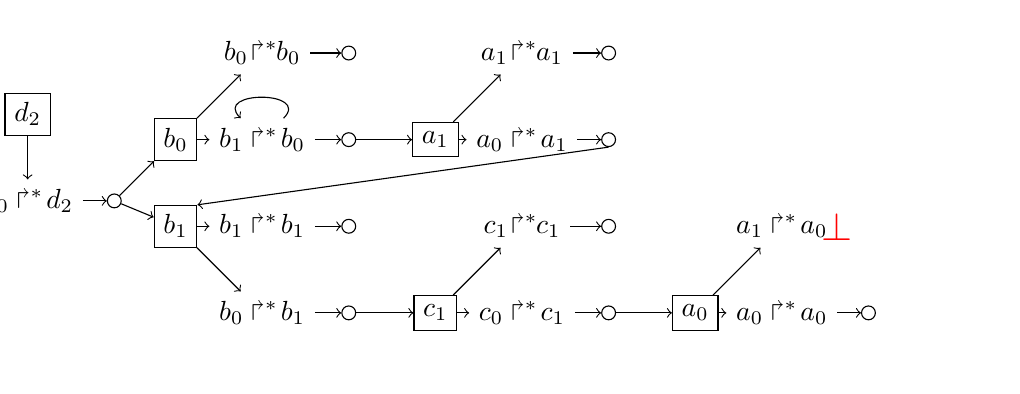
\begin{tikzpicture}[aS,node distance=1.1cm,shorthandon]
\path[use as bounding box] (0,-2.1) rectangle (12.25,2.2);

\node[Aobj] (d02) {$\PHobjectif{d_0}{d_2}$};
\node[Aproc,above of=d02] (d2) {$d_2$};

\node[Asol,right of=d02] (d02s2) {};
\node[Aproc,above right of=d02s2] (b0) {$b_0$};
\node[Aobj,right of=b0] (b10) {$\PHobjectif{b_1}{b_0}$};
\node[Asol,right of=b10] (b10s) {};
\node[Aproc,right of=b10s] (a1) {$a_1$};
\node[Aobj,right of=a1] (a01) {$\PHobjectif{a_0}{a_1}$};
\node[Asol,right of=a01] (a01s) {};

\node[Aproc, below of=b0] (b1) {$b_1$};
\node[Aobj,right of=b1] (b11) {$\PHobjectif{b_1}{b_1}$};
\node[Asol,right of=b11] (b11s) {};
\node[Aobj,below of=b11] (b01) {$\PHobjectif{b_0}{b_1}$};
\node[Asol,right of=b01] (b01s) {};
\node[Aproc,right of=b01s] (c1) {$c_1$};
\node[Aobj,right of=c1] (c01) {$\PHobjectif{c_0}{c_1}$};
\node[Asol,right of=c01] (c01s) {};
\node[Aproc,right of=c01s] (a0) {$a_0$};
\node[Aobj,right of=a0] (a00) {$\PHobjectif{a_0}{a_0}$};
\node[Asol,right of=a00] (a00s) {};

\node[Aobj,above of=b10] (b00) {$\obj{b_0}{b_0}$};
\node[Asol,right of=b00] (b00s) {};
\node[Aobj,above of=a01] (a11) {$\obj{a_1}{a_1}$};
\node[Asol,right of=a11] (a11s) {};
\node[Aobj,above of=c01] (c11) {$\obj{c_1}{c_1}$};
\node[Asol,right of=c11] (c11s) {};
\node[Aobj,above of=a00] (a10) {$\PHobjectif{a_1}{a_0}$};
\node at (a10.east) {\Large\color{red}\textbf{$\bot$}};

\path
  (b10) edge[loop,min distance=5mm] (b10)
 ;
\path
(d02) edge (d02s2) (d02s2) edge (b1) edge (b0)
(a01) edge (a01s) (a01s.south) edge (b1.north east)
(b10) edge (b10s) (b10s) edge (a1)
(b11) edge (b11s)
(a1) edge (a01)
(b0) edge (b10) (b1) edge (b11)
(d2) edge (d02)
;
\path
(b00) edge (b00s)
(b0) edge (b00)
 (b1) edge (b01)
 (b01) edge (b01s) (b01s) edge (c1)
 (c1) edge (c01)
 (c01) edge (c01s) (c01s) edge (a0)
 (a0) edge (a00) (a00) edge (a00s)
;
\path
 (c1) edge (c11) (c11) edge (c11s)
(a0) edge (a10)
(a1) edge (a11)
(a11) edge (a11s)
;

%\node[right of=a01s] {\textbf{\Large\color{darkyellow}Inconc}};

\end{tikzpicture}%
}

% Structure abstraite / Sur-approximation / Non
\def \saono {%
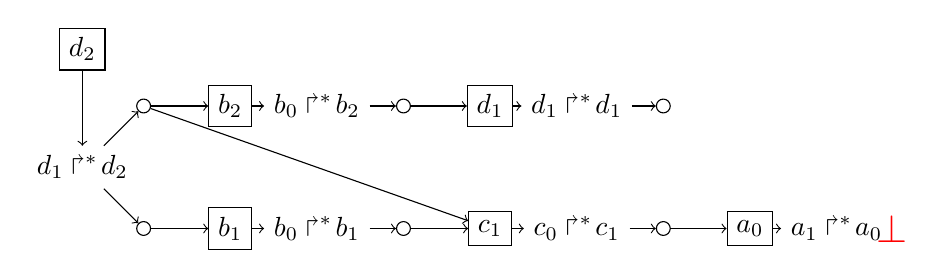
\begin{tikzpicture}[aS,node distance=1.1cm]
%\path[use as bounding box] (-0.5,-2.1) rectangle (10.25,1.15);

\node[Aobj] (d12) {$\PHobjectif{d_1}{d_2}$};
\node[Aproc, above of=d12, node distance=1.5cm] (d2) {$d_2$};
\node[Asol,above right of=d12] (d12s1) {};
\node[Aproc, right of=d12s1] (b2) {$b_2$};
\node[Aobj,right of=b2] (b02) {$\PHobjectif{b_0}{b_2}$};
\node[Asol,right of=b02] (b02s) {};
\node[Aproc,right of=b02s] (d1) {$d_1$};
\node[Aobj,right of=d1] (d11) {$\PHobjectif{d_1}{d_1}$};
\node[Asol,right of=d11] (d11s) {};

\node[Asol,below right of=d12] (d12s2) {};
\node[Aproc, right of=d12s2] (b1) {$b_1$};
\node[Aobj,right of=b1] (b01) {$\PHobjectif{b_0}{b_1}$};
\node[Asol,right of=b01] (b01s) {};
\node[Aproc,right of=b01s] (c1) {$c_1$};
\node[Aobj,right of=c1] (c01) {$\PHobjectif{c_0}{c_1}$};
\node[Asol,right of=c01] (c01s) {};
\node[Aproc,right of=c01s] (a0) {$a_0$};
\node[Aobj,right of=a0] (a10) {$\PHobjectif{a_1}{a_0}$};
\node at (a10.east) {\Large\color{red}\textbf{$\bot$}};

\path
(d2) edge (d12)
(d12) edge (d12s1) edge (d12s2) (d12s1) edge (b2) edge (c1) (d12s2) edge (b1)
(b01) edge (b01s) (b01s) edge (c1)
(b02) edge (b02s) (b02s) edge (d1)
(c01) edge (c01s) (c01s) edge (a0)
(d11) edge (d11s)
(a0) edge (a10)
(b1) edge (b01)
(b2) edge (b02)
(c1) edge (c01)
(d1) edge (d11)
;
%\only<\value{anim1}>{ \node[above right of=c01s] {\textbf{\Large\color{red}No}};}
\end{tikzpicture}%
}

% Structure abstraite / Sur-approximation / Inconclusif
\def \saoinconc {%
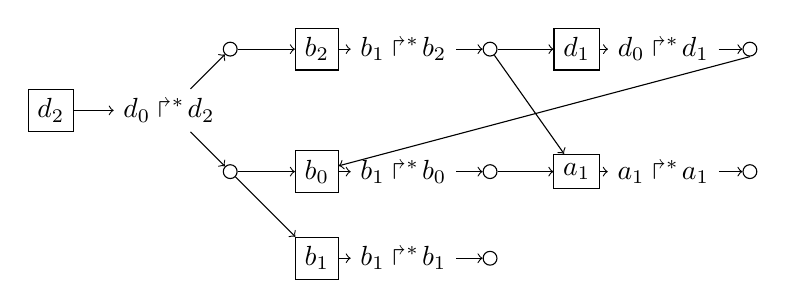
\begin{tikzpicture}[aS,node distance=1.1cm]
%\path[use as bounding box] (-0.5,-2.1) rectangle (10.25,1.15);

\node[Aobj] (d02) {$\PHobjectif{d_0}{d_2}$};
\node[Aproc, left of=d02, node distance=1.5cm] (d2) {$d_2$};
\node[Asol,above right of=d02] (d02s1) {};

\node[Aproc, right of=d02s1] (b2) {$b_2$};
\node[Aobj,right of=b2] (b12) {$\PHobjectif{b_1}{b_2}$};
\node[Asol,right of=b12] (b12s) {};
\node[Aproc,right of=b12s] (d1) {$d_1$};
\node[Aobj,right of=d1] (d01) {$\PHobjectif{d_0}{d_1}$};
\node[Asol,right of=d01] (d01s) {};

\node[Asol,below right of=d02] (d02s2) {};
\node[Aproc, right of=d02s2] (b0) {$b_0$};
%\node<\tokp>[orange, thick, Aproc, right of=d02s2] (b0) {$b_0$};
\node[Aobj,right of=b0] (b10) {$\PHobjectif{b_1}{b_0}$};
\node[Asol,right of=b10] (b10s) {};
\node[Aproc,right of=b10s] (a1) {$a_1$};
%\node<\tokp>[orange, thick, Aproc,right of=b10s] (a1) {$a_1$};
\node[Aobj,right of=a1] (a11) {$\PHobjectif{a_1}{a_1}$};
\node[Asol,right of=a11] (a11s) {};

\node[Aproc, below of=b0] (b1) {$b_1$};
\node[Aobj,right of=b1] (b11) {$\PHobjectif{b_1}{b_1}$};
\node[Asol,right of=b11] (b11s) {};

\path
(d2) edge (d02)
(d02) edge (d02s1) edge (d02s2) (d02s1) edge (b2) (d02s2) edge (b1) edge (b0)
(a11) edge (a11s)
(b10) edge (b10s) (b10s) edge (a1)
(b11) edge (b11s)
(b12) edge (b12s) (b12s) edge (d1) edge (a1)
(d01) edge (d01s) (d01s.south) edge (b0)
(a1) edge (a11)
(b0) edge (b10) (b1) edge (b11) (b2) edge (b12)
(d1) edge (d01)
;
%\node[below right of=d01s] {\textbf{\Large\color{yellow}Inconc}};
\end{tikzpicture}%
}



% Structure abstraite / Sur-approximation / Inconclusif / Avec processus-clefs
\def \saoinconckp {%
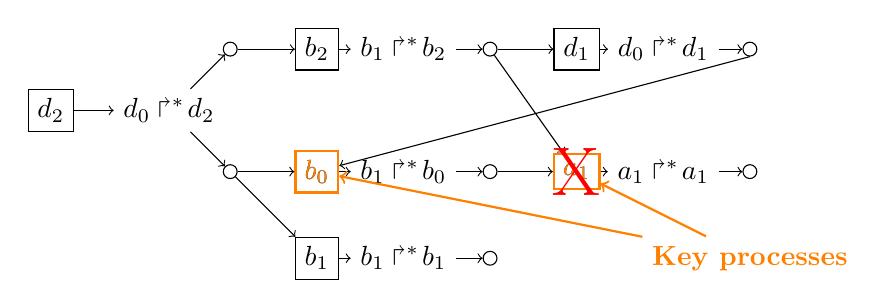
\begin{tikzpicture}[aS,node distance=1.1cm]
%\path[use as bounding box] (-0.5,-2.1) rectangle (10.25,1.15);

\node[Aobj] (d02) {$\PHobjectif{d_0}{d_2}$};
\node[Aproc, left of=d02, node distance=1.5cm] (d2) {$d_2$};
\node[Asol,above right of=d02] (d02s1) {};

\node[Aproc, right of=d02s1] (b2) {$b_2$};
\node[Aobj,right of=b2] (b12) {$\PHobjectif{b_1}{b_2}$};
\node[Asol,right of=b12] (b12s) {};
\node[Aproc,right of=b12s] (d1) {$d_1$};
\node[Aobj,right of=d1] (d01) {$\PHobjectif{d_0}{d_1}$};
\node[Asol,right of=d01] (d01s) {};

\node[Asol,below right of=d02] (d02s2) {};
\node<-2,4->[Aproc, right of=d02s2] (b0) {$b_0$};
\node<3>[orange, thick, Aproc, right of=d02s2] (b0) {$b_0$};
\node[Aobj,right of=b0] (b10) {$\PHobjectif{b_1}{b_0}$};
\node[Asol,right of=b10] (b10s) {};
\node<-2,4->[Aproc,right of=b10s] (a1) {$a_1$};
\node<3>[orange, thick, Aproc,right of=b10s] (a1) {$a_1$};
\node[Aobj,right of=a1] (a11) {$\PHobjectif{a_1}{a_1}$};
\node[Asol,right of=a11] (a11s) {};

\node[Aproc, below of=b0] (b1) {$b_1$};
\node[Aobj,right of=b1] (b11) {$\PHobjectif{b_1}{b_1}$};
\node[Asol,right of=b11] (b11s) {};

\path
(d2) edge (d02)
(d02) edge (d02s1) edge (d02s2) (d02s1) edge (b2) (d02s2) edge (b1) edge (b0)
(a11) edge (a11s)
(b10) edge (b10s) (b10s) edge (a1)
(b11) edge (b11s)
(b12) edge (b12s) (b12s) edge (d1) edge (a1)
(d01) edge (d01s) (d01s.south) edge (b0)
(a1) edge (a11)
(b0) edge (b10) (b1) edge (b11) (b2) edge (b12)
(d1) edge (d01)
;

\uncover<3>{
\node[orange, font=\bfseries,below of=a11s] (kp) {Key processes};
\path[orange, thick]
        (kp) edge (a1)
        (kp) edge (b0)
;}
%\node[below right of=d01s] {\textbf{\Large\color{yellow}Inconc}};

\node<4->[font=\Huge,red] at (a1) {X};

\end{tikzpicture}%
}
\newcommand{\cmodels}{\bigskip
\quad\tval{\ex{egfr20}}: \tcite{Epidermal Growth Factor Receptor, by Özgür Sahin \textit{et al.}}\\
\quad\tval{\ex{egfr104}}: \tcite{Epidermal Growth Factor Receptor, by Regina Samaga \textit{et al.}}\\
\quad\tval{\ex{tcrsig40}}: \tcite{T-Cell Receptor Signaling, by Steffen Klamt \textit{et al.}}\\
\quad\tval{\ex{tcrsig94}}: \tcite{T-Cell Receptor Signaling, by Julio Saez-Rodriguez \textit{et al.}}\\}

\section{Introduction}
% Diapo d'intro

\begin{frame}[c]
  \frametitle{Context and Aims}

\tval{MeForBio} team: Algebraic modeling to study complex dynamical biological systems

%\bigskip
\begin{center}
  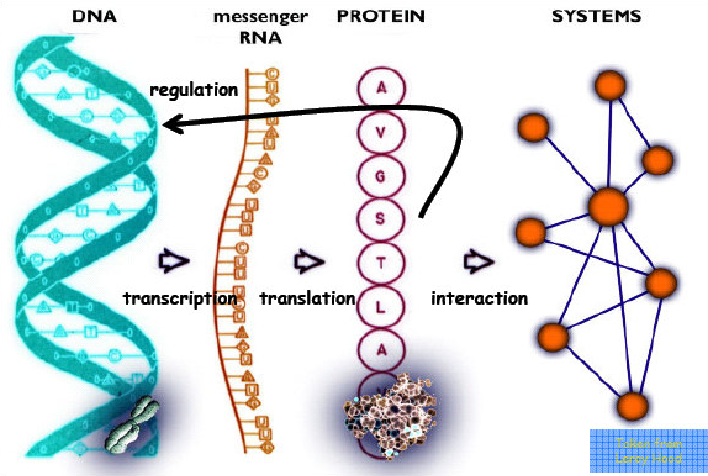
\includegraphics[height=3.5cm]{figs/dnascheme_white.png}
\end{center}

\pause
\begin{enumerate}[1)]
  \item Two main models
  \begin{itemize}
    \item Historical model: \tval{Biological Regulatory Network (René Thomas)}
    \item New developed model: \tval{Process Hitting}
  \end{itemize}

\medskip
  \item Allow efficient translation from Process Hitting to BRN
\end{enumerate}

\end{frame}


\section{Frameworks Definitions}
\subsection{The Process Hitting framework}
%% Définition du Process Hitting + sortes coopératives

\begin{frame}[t]
  \frametitle{The Process Hitting modeling}
  \framesubtitle{\tcite{\cpmrtcsb}}

% 1 : Sortes
\only<1>{
\tikzstyle{process}=[circle,minimum size=15pt,font=\footnotesize,inner sep=1pt]
\tikzstyle{tick label}=[color=white, font=\footnotesize]
\tikzstyle{tick}=[transparent]
\tikzstyle{hit}=[transparent]
\tikzstyle{selfhit}=[transparent, min distance=30pt,curve to]
\tikzstyle{bounce}=[transparent]
\tikzstyle{hlhit}=[transparent]
\begin{center}\scalebox{\scaleex}{
\begin{tikzpicture}
\exphdef
\end{tikzpicture}
}\end{center}
}

% 2 : Processus
\only<2>{
\tikzstyle{process}=[circle,draw,minimum size=15pt,font=\footnotesize,inner sep=1pt]
\tikzstyle{tick label}=[font=\footnotesize]
\tikzstyle{tick}=[densely dotted]
\tikzstyle{hit}=[transparent]
\tikzstyle{selfhit}=[transparent, min distance=30pt,curve to]
\tikzstyle{bounce}=[transparent]
\tikzstyle{hlhit}=[transparent]
\begin{center}\scalebox{\scaleex}{
\begin{tikzpicture}
\exphdef
\end{tikzpicture}
}\end{center}
}

% 3 : États
\only<3>{
\tikzstyle{hit}=[transparent]
\tikzstyle{selfhit}=[transparent, min distance=30pt,curve to]
\tikzstyle{bounce}=[transparent]
\tikzstyle{hlhit}=[transparent]
\begin{center}\scalebox{\scaleex}{
\begin{tikzpicture}
\exphdef

\TState{3}{a_0,b_1,z_0}
\end{tikzpicture}
}\end{center}
}

% 4 : Actions
\only<4->{
\tikzstyle{tick}=[densely dotted]
\tikzstyle{hit}=[->,>=angle 45]
\tikzstyle{selfhit}=[min distance=30pt,curve to]
\tikzstyle{bounce}=[densely dotted,>=stealth',->]
\tikzstyle{hlhit}=[very thick]
\begin{center}\scalebox{\scaleex}{
\begin{tikzpicture}
\exphdef
\TState{4}{a_0,b_1,z_0}
\TState{5}{a_0,b_1,z_1}
\TState{6}{a_1,b_1,z_1}
\TState{7}{a_1,b_1,z_2}
\end{tikzpicture}
}\end{center}
}

\medskip
\begin{liste}
  \item \tval{Sorts}: components \qex{$a$, $b$, $z$}
\pause[2]
  \item \tval{Processes}: local states / levels of expression \qex{$z_0$, $z_1$, $z_2$}
\pause[3]
  \item \tval{States}: sets of active processes%
  \only<3-4>{\qex{$\PHetat{a_0, b_1, z_0}$}}%
  \only<5>{\qex{$\PHetat{a_0, b_1, z_1}$}}%
  \only<6>{\qex{$\PHetat{a_1, b_1, z_1}$}}%
  \only<7>{\qex{$\PHetat{a_1, b_1, z_2}$}}%
\pause[4]
  \item \tval{Actions}: dynamics \qex{\only<4>{\underline}{$\PHfrappe{b_1}{z_0}{z_1}$}, \only<4-5>{\underline}{$\PHfrappe{a_0}{a_0}{a_1}$}, \only<6>{\underline}{$\PHfrappe{a_1}{z_1}{z_2}$}}
\end{liste}
\end{frame}



\begin{frame}
  \frametitle{Adding cooperations}
  \framesubtitle{\tcite{\cpmrtcsb}}

\begin{center}\scalebox{\scaleex}{
\begin{tikzpicture}
\exphcoop
\end{tikzpicture}
}\end{center}

\medskip
\only<-14>{
\begin{liste}
  \item How to introduce some \tval{cooperation} between sorts? \qex{$\PHfrappe{a_1 \wedge b_0}{z_1}{z_2}$}
\pause[4]
  \item Solution: a \tval{cooperative sort} \qex{$ab$} \only<12->{\quad to express \qex{$a_1 \wedge b_0$}}
\pause[8]
  \item Constraint: each configuration is represented by one process \qex{$\PHetat{a_1,b_0} \pause[11]\Rightarrow ab_{10}$}
\pause[14]
  \item Advantage: regular sort; drawbacks: complexity, temporal shift
\end{liste}}
\end{frame}



\begin{frame}[c]
  \frametitle{The Process Hitting modeling}

\begin{itemize}
  \item \tval{Dynamic} modeling with an \tval{atomistic} point of view
  \begin{fleches}
    \item Independent actions
    \item Cooperation modeled with cooperative sorts
  \end{fleches}

  \smallskip
  \item Efficient \tval{static analysis}
  \begin{fleches}
    \item Reachability of a process can be computed in \tval{polynomial time}\\
          \quad in the number of sorts
  \end{fleches}

  \smallskip
  \item Useful for the study of \tval{large biological models}
  \begin{fleches}
    \item Up to hundreds of sorts
  \end{fleches}

  \smallskip
  \item (Future) extensions
  \begin{fleches}
    \item Actions with priorities
    \item Continuous time with clocks?
  \end{fleches}
\end{itemize}

\end{frame}


\subsection{Thomas Modeling}
%% Définition du modèle de Thomas

\colorlet{light}{colorgray}

\begin{frame}
  \frametitle{Biological Regulatory Network (Thomas' modeling)}
  \framesubtitle{\tcite{\crcbmfma}}

\begin{tabular}{cccc}

\begin{tikzpicture}[grn]
\path[use as bounding box] (-0.7,-0.3) rectangle (2.5,2);
% Nœuds noirs
\only<1,3->{
  \node[inner sep=0] (z) at (2,0.75) {z};
  \node[inner sep=0] (a) at (0,1.5) {a};
  \node[inner sep=0] (b) at (0,0) {b};
  \path
    node[elabel, below=-1em of a] {$0..1$}
    node[elabel, below=-1em of b] {$0..1$}
    node[elabel, below=-1em of z] {$0..2$};}
% Nœuds grisés
\only<2>{
  \node[inner sep=0,light] (z) at (2,0.75) {z};
  \node[inner sep=0,light] (a) at (0,1.5) {a};
  \node[inner sep=0,light] (b) at (0,0) {b};
  \path
    node[elabel, below=-1em of a,light] {$0..1$}
    node[elabel, below=-1em of b,light] {$0..1$}
    node[elabel, below=-1em of z,light] {$0..2$};}

% Arcs colorés
\only<1,4->{\path
  (a) edge[inh,loop left=10] node[elabel, left] {$1-$} (a)
  (a) edge[act] node[elabel, above=-2pt] {$1+$} (z)
  (b) edge[inh] node[elabel, below=-2pt] {$1-$} (z);}
% Arcs grisés
\only<2-3>{\path
  (a) edge[inhgray,loop left=10] node[elabel, left,light] {$1-$} (a)
  (a) edge[actgray] node[elabel, above=-2pt,light] {$1+$} (z)
  (b) edge[inhgray] node[elabel, below=-2pt,light] {$1-$} (z);}
\end{tikzpicture}
&%
\only<2-4>{\color{light}}%
\begin{tabular}[b]{c|c|c}
  \multicolumn{2}{c|}{$\omega$} & \multirow{2}{*}{$k_{z, \omega}$} \\
\cline{1-2}
  $a$ & $b$ & \\
\hline
  $-$ & $+$ & $1$ \\
  $-$ & $-$ & $0$ \\
  $+$ & $+$ & $2$ \\
  \only<6>{\color{red}}$+$ & \only<6>{\color{red}}$-$ & \only<6>{\color{red}}$1$
\end{tabular}
%\begin{tabular}[b]{c|c}
%  $\omega$ & $k_{z, \omega}$ \\
%\hline
%  $\emptyset$ & $1$ \\
%  $\{b\}$ & $0$ \\
%  \only<7-8>{\color{red}}$\{a\}$ & \only<7-8>{\color{red}}$2$ \\
%  $\{a;b\}$ & $1$
%\end{tabular}
~~~~&
\only<2-4>{\color{light}}%
\begin{tabular}[b]{c|c}
  $\omega$ & \multirow{2}{*}{$k_{a, \omega}$} \\
\cline{1-1}
  $a$ & \\
\hline
  $+$ & $1$ \\
  $-$ & $0$
\end{tabular}
%\begin{tabular}[b]{c|c}
%  $\omega$ & $k_{a, \omega}$ \\
%\hline
%  $\emptyset$ & $1$ \\
%  $\{a\}$ & $0$
%\end{tabular}
&
\only<2-4>{\color{light}}%
\begin{tabular}[b]{cc}
  & $k_{b, \omega}$ \\
\cline{2-2}
  & $1$
\end{tabular}
%\begin{tabular}[b]{c|c}
%  $\omega$ & $k_{b, \omega}$ \\
%\hline
%  $\emptyset$ & $1$
%\end{tabular}
\\
\only<2-4>{$\underbrace{\text{\hspace{3cm}}}_{\text{Interaction Graph}}$}%
&
\multicolumn{3}{r}{\only<5->{$\underbrace{\text{\hspace{6.5cm}}}_\text{Parametrization}$}}
\end{tabular}

\bigskip
% Historical model...
\only<1>{

\bigskip
Proposed by René Thomas in 1973, several extensions since then
\medskip
\begin{liste}
  \item \tval{Historical bio-informatics model} for studying genes interactions
  \item Widely used and well-adapted to represent dynamic gene systems
\end{liste}
}

% Interaction Graph
\only<2-4>{
\tval{Interaction Graph}: structure of the system (genes \& interactions)

\pause[3]
\medskip
\begin{liste}
  \item \tval{Nodes}: genes
  \begin{fleches}
    \item Name \qex{$a$, $b$, $z$}
    \item Possible values (levels of expression) \qex{$0..1$, $0..2$}
  \end{fleches}
\pause[4]
  \item \tval{Edges}: interactions
  \begin{fleches}
    \item Threshold \qex{$1$}
    \item Type (activation or inhibition) \qex{$+$ / $-$}
  \end{fleches}
\end{liste}
}

% Parametrization
\only<5->{
\medskip
\tval{Parametrization}: strength of the influences (cooperations)

\medskip
\begin{liste}
  \item Maps of tendencies for each gene
  \begin{fleches}
    \item To any \tval{influences of predecessors} \qex{$\omega$}
    \item Corresponds a \tval{parameter} \qex{$k_{x,\omega}$}
  \end{fleches}
\pause[6]
\medskip
  \item \ex{“$k_{z, \{a^+, b^-\}} = 1$”} \quad means: \qex{“$z$ tends to $2$ when activated by $a$ and inhibited by $b$”}
%  \item \ex{“$k_{z, \{a\}} = [2;2]$”} \quad means: \qex{“$z$ tends to \only<7>{$[2;2]$}\only<8->{$2$} when $a \only<7>{\geq}\only<8->{=} 1$ and $b \only<7>{< 1}\only<8->{= 0}$”}
\end{liste}
%\pause[10]
}\end{frame}



\begin{frame}
  \frametitle{Biological Regulatory Network (Thomas' modeling)}
  \framesubtitle{\tcite{\crcbmfma}}

\begin{tabular}{cccc}

\begin{tikzpicture}[grn]
\path[use as bounding box] (-0.7,-0.3) rectangle (2.5,2);
\node[inner sep=0] (z) at (2,0.75) {z};
\node[inner sep=0] (a) at (0,1.5) {a};
\node[inner sep=0] (b) at (0,0) {b};
\path
  node[elabel, below=-1em of a] {$0..1$}
  node[elabel, below=-1em of b] {$0..1$}
  node[elabel, below=-1em of z] {$0..2$};
\path
  (a) edge[inh,loop left=10] node[elabel, left] {$1-$} (a)
  (a) edge[act] node[elabel, above=-2pt] {$1+$} (z)
  (b) edge[inh] node[elabel, below=-2pt] {$1-$} (z);
\end{tikzpicture}
&
\begin{tabular}[b]{c|c|c}
  \multicolumn{2}{c|}{$\omega$} & \multirow{2}{*}{$k_{z, \omega}$} \\
\cline{1-2}
  $a$ & $b$ & \\
\hline
  $-$ & $+$ & $1$ \\
  $-$ & $-$ & $0$ \\
  $+$ & $+$ & $2$ \\
  $+$ & $-$ & $1$
\end{tabular}
~~~~&
\begin{tabular}[b]{c|c}
  $\omega$ & \multirow{2}{*}{$k_{a, \omega}$} \\
\cline{1-1}
  $a$ & \\
\hline
  $+$ & $1$ \\
  $-$ & $0$
\end{tabular}
&
\begin{tabular}[b]{cc}
   & $k_{b, \omega}$ \\
\cline{2-2}
   & $1$
\end{tabular}
\\
\multicolumn{4}{r}{$\underbrace{\text{\hspace{10.1cm}}}_{\text{Biological Regulatory Network}}$}
\end{tabular}

\bigskip

\begin{itemize}
  \item[\f] All needed information to run the model or study its dynamics:
  \begin{itemize}\normalsize
    \item Build the State Graph
    \item Find reachability properties, fixed points, attractors
    \item Other properties...
  \end{itemize}
\end{itemize}

\begin{itemize}
  \item[\f] \tval{Strengths}: well adapted for the study of biological systems
  \item[\f] \tval{Drawbacks}: inherent complexity; needs the full\\
    \quad \quad specification of cooperations
\end{itemize}
\end{frame}


\section{Translating a Process Hitting into a BRN}
%% Introduction à la traduction

\begin{frame}[c]
  \frametitle{Inferring a BRN with Thomas' parameters}
  \framesubtitle{~}

\begin{center}
\scalebox{\scaleinf}{
\begin{tikzpicture}
\path[use as bounding box] (-0.5,-0.8) rectangle (6.5,4);
\exphinfblack
\end{tikzpicture}
}
\end{center}

\begin{center}
\begin{tikzpicture}
\path[use as bounding box] (1,1) rectangle (4,1.5);
\only<2->{
  \path[draw] (1, 1.8) edge[->,draw,very thick] node[left=3pt,circle,draw=black,outer sep=2pt,minimum size=15pt,text=black] {1} (0, 0);}

\only<3->{
\node[circle,draw=black,inner sep=0,minimum size=5pt,fill=black] (s2) at (2,0.7) {};
\node[left=4pt of s2,circle,draw=black,outer sep=2pt,minimum size=15pt,text=black,very thick] (e2) at (2,0.8) {2};
\path[draw] (2.25, 1.8) edge[draw,very thick] (s2);
\path[draw] (1, -0.25) edge[draw,very thick] (s2);
\path[draw] (s2) edge[->,draw,very thick] (3.75, 0);}
\end{tikzpicture}
\end{center}

\begin{columns}
\begin{column}{0.6\textwidth}

\begin{center}
\begin{tikzpicture}[grn]
\path[use as bounding box] (0.5,-0.5) rectangle (2,1.5);
% Gènes noirs
\only<2->{
  \node[inner sep=0] (a) at (0,1.5) {a};
  \node[inner sep=0] (b) at (0,0) {b};
  \node[inner sep=0] (z) at (2,0.75) {z};}
% Gènes gris
\only<1>{
  \node[inner sep=0,colorgray] (a) at (0,1.5) {a};
  \node[inner sep=0,colorgray] (b) at (0,0) {b};
  \node[inner sep=0,colorgray] (z) at (2,0.75) {z};}

% Arcs colorés
\only<2->{
  \path (a) edge[act] node[elabel,above=-2pt] {$1+$} (z);
  \path (b) edge[inh] node[elabel,below=-2pt] {$1-$} (z);}
% Arcs grisés
\only<1>{
  \path (a) edge[actgray] node[elabel,above=-2pt,colorgray] {$1+$} (z);
  \path (b) edge[inhgray] node[elabel,below=-2pt,colorgray] {$1-$} (z);}
\end{tikzpicture}
\end{center}

\end{column}
\begin{column}{0.4\textwidth}

\only<1-2>{\color{colorgray}}
\begin{tabular}[b]{c|c|c}
  \multicolumn{2}{c|}{$\omega$} & \multirow{2}{*}{$k_{z, \omega}$} \\
\cline{1-2}
  $a$ & $b$ & \\
\hline
  $-$ & $+$ & $1$ \\
  $-$ & $-$ & $0$ \\
  $+$ & $+$ & $2$ \\
  $+$ & $-$ & $1$
\end{tabular}

\end{column}
\end{columns}


\end{frame}

\subsection{Interaction Graph Inference}
%% Inférence du Graphe des Interactions



\begin{frame}
  \frametitle{Inferring the Interaction Graph}
  \framesubtitle{\tcite{\cfpimrcmsb}}

\begin{columns}
\begin{column}{0.65\textwidth}

\begin{center}\scalebox{\scaleinf}{
\begin{tikzpicture}
\path[use as bounding box] (-0.5,-0.8) rectangle (6.5,2.8);
\exphinf

% Processus marqués
\only<4-9>{\node[current process,fill=colorb] (hb_0) at (b_0.center) {};}
\only<5-9>{
  \node[current process,fill=colora1] (ha_1) at (a_1.center) {};
  \node[current process,fill=colora1] (hab_2) at (ab_2.center) {};}
\only<6-9>{
  \node[current process,fill=colora1] (hz_2) at (z_2.center) {};}
\only<7-9>{
  \node[current process,fill=colora0] (ha_0) at (a_0.center) {};
  \node[current process,fill=colora0] (hab_0) at (ab_0.center) {};}
\only<8-9>{
  \node[current process,fill=colora0] (hz_0) at (z_0.center) {};}

\only<10->{\node[current process,fill=colorb] (hb_1) at (b_1.center) {};}
\only<10->{
  \node[current process,fill=colora1] (ha_1) at (a_1.center) {};
  \node[current process,fill=colora1] (hab_3) at (ab_3.center) {};
  \node[current process,fill=colora0] (ha_0) at (a_0.center) {};
  \node[current process,fill=colora0] (hab_1) at (ab_1.center) {};}
\only<11->{
  \node[current process,fill=colora1] (hz_1) at (z_1.center) {};
  \node[current process,fill=colora0,inner sep=0,minimum size=7pt,draw=none] (hz_1bis) at (z_1.center) {};}

% Actions mises en valeur
\only<5-6>{
  \THit{ab_2}{}{z_1}{.north west}{z_2}
  \THit{ab_2}{}{z_0}{.west}{z_1}
  \path[bounce,bend left] \TBounce{z_1}{}{z_2}{.south} \TBounce{z_0}{}{z_1}{.south} ;}
\only<7-8>{
  \THit{ab_0}{}{z_2}{.west}{z_1}
  \THit{ab_0}{}{z_1}{.south west}{z_0}
  \path[bounce,bend right] \TBounce{z_2}{}{z_1}{.north} \TBounce{z_1}{}{z_0}{.north} ;}
\only<10->{
  \THit{ab_3}{}{z_2}{.west}{z_1}
  \THit{ab_3}{}{z_0}{.west}{z_1}
  \THit{ab_1}{}{z_2}{.west}{z_1}
  \THit{ab_1}{}{z_0}{.west}{z_1}
  \path[bounce,bend left] \TBounce{z_2}{bend right}{z_1}{.north} \TBounce{z_0}{}{z_1}{.south} ;}

\end{tikzpicture}
}\end{center}

\end{column}
\begin{column}{0.45\textwidth}

\begin{center}
\begin{tikzpicture}[grn]
\path[use as bounding box] (1,-0.5) rectangle (2.5,1.5);
% Gènes noirs
\only<1->{\node[inner sep=0] (a) at (0,1.5) {a};}
\only<1-3>{\node[inner sep=0] (b) at (0,0) {b};}
\only<1->{\node[inner sep=0] (z) at (2,0.75) {z};}
%\only<1-2>{\path node[elabel, below=-1em of a] {$0..1$}; \path node[elabel, below=-1em of b] {$0..1$}; \path node[elabel, below=-1em of z] {$0..2$};}
% Gènes gris
%\only<3>{\node[colorgray,inner sep=0] (a) at (0,1.5) {a};}
\only<4->{\node[colorgray,inner sep=0] (b) at (0,0) {b};}

%\newcolumntype{M}[1]{>{\raggedright}m{#1}}

% Arc noir
\only<2-12>{\path (a) edge[inf] node[elabel,above right=-2.4em,font=\scriptsize] {\begin{tabular*}{3cm}{c}%
$\color{white}\left\{\color{black}\text{\begin{tabular*}{1.7cm}{l}%
  $\only<10->{\{b = 1\} \only<15>{\phantom{\Rightarrow \sim}}\only<12->{\Rightarrow {\color{exanswer}\sim}}}$\tabularnewline%
  $\only<4->{\{b = 0\} \only<9->{\Rightarrow {\color{exanswer}1+}}}$%
\end{tabular*}}\only<-16>{\right.}\only<17->{\right\}\textcolor{exanswer}{1+}}$%
\end{tabular*}} (z) ;}
\only<2-3>{\path (b) edge[inf] node[elabel, below=-2pt] {$\only<99->{-\!\only<1->{1}}$} (z) ;}
% Arc coloré
\only<13->{\path (a) edge[act,very thick,notsodarkgreen] node[elabel,above right=-2.4em,font=\scriptsize] {\begin{tabular*}{3cm}{c}%
$\color{white}\left\{\color{black}\text{\begin{tabular*}{1.7cm}{l}%
  $\only<10->{\{b = 1\} \only<11>{\phantom{\Rightarrow \sim}}\only<12->{\Rightarrow {\color{exanswer}\sim}}}$\tabularnewline%
  $\only<4->{\{b = 0\} \only<9->{\Rightarrow {\color{exanswer}1+}}}$%
\end{tabular*}}\only<13->{\right\}\textcolor{exanswer}{1+}}$%
\end{tabular*}} (z) ;}
% Arcs gris
%\only<3>{\path (a) edge[inf,draw=colorgray,fill=colorgray] node[colorgray,elabel, above=-2pt] {$\only<1>{+\!\only<2->{1}}$} (z) ;}
\only<4->{\path (b) edge[inf,draw=colorgray,fill=colorgray] node[colorgray,elabel, below=-2pt] {$\only<1>{-\!\only<1->{1}}$} (z) ;}
\end{tikzpicture}
\end{center}

\end{column}
\end{columns}

\bigskip

% Méthode
\pause[3]
\f \tval{Exhaustive search in all possible configurations}

\pause
\begin{enumerate}[1.]
  \item Pick one regulator [\ex{$a$}], and choose an active process for all the others [\ex{$b_0$}].
\pause
  \item Change the active process of this regulator [\ex{$a_0$}, \ex{$a_1$}] and watch the \tval{focal processes}.
\pause[9]
  \item Conclude locally: ($\textcolor{colora0font}{a_0} \Rsh \textcolor{colora1font}{a_1} \Rightarrow \textcolor{colora0font}{z_0} \Rsh \textcolor{colora1font}{z_2}$)
      $\Rightarrow \text{activation (}\textcolor{exanswer}{+}\text{) \& threshold = \ex{$1$}}$.
\pause
  \item Iterate \only<13->{and conclude globally.}
\end{enumerate}

\pause[14]
\smallskip
Problematic cases:\\
\smallskip
$\left.\text{\begin{tabular}{l}
  \f No focal processes (cycle)\\
  \f Opposite influences (\ex{$+$} \& \ex{$-$})
 \end{tabular}}\right\} \Rightarrow \text{ Unsigned edge}$
\end{frame}

\subsection{Parametrization Inference}
%% Inférence de la Paramétrisation

\begin{frame}
  \frametitle{Inferring Parameters}
  \framesubtitle{\tcite{\cpmrtcsb}}

\begin{columns}
\begin{column}{0.5\textwidth}

\only<1-5>{
\begin{center}
\scalebox{\scaleinf}{
\begin{tikzpicture}
\path[use as bounding box] (-0.5,-0.8) rectangle (6.5,2.8);
\exphinf

% Processus mis en valeur
\only<2->{
  \node[current process,fill=colorb] (hb_1) at (b_1.center) {};
  \node[current process,fill=colorb] (ha_1) at (a_1.center) {};}
\only<2->{
  \node[current process,fill=colorb] (hab_3) at (ab_3.center) {};}
\only<3->{
  \node[current process,fill=colorb] (hz_1) at (z_1.center) {};}

% Actions mises en valeur
\only<3->{
  \THit{ab_3}{}{z_2}{.west}{z_1}
  \THit{ab_3}{}{z_0}{.west}{z_1}
  \path[bounce,bend left] \TBounce{z_2}{bend right}{z_1}{.north} \TBounce{z_0}{}{z_1}{.south};}
\end{tikzpicture}
}
\end{center}
}

\only<6->{
\begin{center}
\scalebox{\scaleinf}{
\begin{tikzpicture}
\path[use as bounding box] (-0.5,-0.8) rectangle (6.5,2.8);
\exphinfprojssc

% Processus mis en valeur
\only<2->{
  \node[current process,fill=colorb] (hb_1) at (b_1.center) {};
  \node[current process,fill=colorb] (ha_1) at (a_1.center) {};}

% Actions mises en valeur
\only<2->{
  \THit{a_1}{}{z_0}{.west}{z_1}
  \THit{a_1}{}{z_1}{.north west}{z_2}
  \THit{b_1}{}{z_1}{.south west}{z_0}
  \THit{b_1}{}{z_2}{.west}{z_1}
  \path[bounce,bend left] \TBounce{z_0}{}{z_1}{.south} \TBounce{z_1}{}{z_2}{.south}
    \TBounce{z_1}{bend right}{z_0}{.north} \TBounce{z_2}{bend right}{z_1}{.north} ;}

\end{tikzpicture}
}
\end{center}
}

\end{column}
\begin{column}{0.2\textwidth}

\begin{center}
\begin{tikzpicture}[grn]
\path[use as bounding box] (0.5,-0.5) rectangle (2,1.5);
% Gènes noirs
  \node[inner sep=0] (a) at (0,1.5) {a};
  \node[inner sep=0] (b) at (0,0) {b};
  \node[inner sep=0] (z) at (2,0.75) {z};
% Arcs colorés
  \path (a) edge[act] node[elabel,above=-2pt] {$1+$} (z) ;
  \path (b) edge[inh] node[elabel,below=-2pt] {$1-$} (z) ;
\end{tikzpicture}
\end{center}

\end{column}
\begin{column}{0.25\textwidth}

\only<1-5>{
\begin{tabular}{c|c|c}
%  $\omega$ & $k_{z, \omega}$ \\
%\hline
  \multicolumn{2}{c|}{$\omega$} & \multirow{2}{*}{$k_{z, \omega}$} \\
\cline{1-2}
  $a$ & $b$ & \\
\hline
  \only<2->{\color{colorgray}}$-$ & \only<2->{\color{colorgray}}$+$ & \\
  \only<2->{\color{colorgray}}$-$ & \only<2->{\color{colorgray}}$-$ & \\
  \only<2->{\color{colorgray}}$+$ & \only<2->{\color{colorgray}}$+$ & \\
  \only<1>{$+$}\only<2->{\redex{$+$}} & \only<1>{$-$}\only<2->{\redex{$-$}} & \uncover<4->{\redex{$1$}}
\end{tabular}
}

\only<6->{
\begin{tabular}{c|c|c}
%  $\omega$ & $k_{z, \omega}$ \\
%\hline
  \multicolumn{2}{c|}{$\omega$} & \multirow{2}{*}{$k_{z, \omega}$} \\
\cline{1-2}
  $a$ & $b$ & \\
\hline
  $-$ & $+$ & \redex{\textit{?}} \\ %\textcolor{lightgray}{\textit{?}} \\
  $-$ & $-$ & $0$ \\
  $+$ & $+$ & $2$ \\
  $+$ & $-$ & \redex{\textit{?}} %\textcolor{lightgray}{\textit{?}}
\end{tabular}
}

\end{column}
\end{columns}

\bigskip
\pause[2]
\begin{enumerate}[1.]
  \item For each configuration of resources \quad [\ex{$\omega = \{a^+, b^-\}$}]\\
\pause
        find the \tval{focal processes}.\pause[4] If possible, conclude. \quad [$\ex{k_{z,\{a^+, b^-\}} = 1}$]
\pause[5]
 \item[] Inconclusive cases:
  \begin{itemize}
    \item[--] Behavior cannot be represented as a BRN
    \item[--] Lack of cooperation (no focal processes)
  \end{itemize}
\medskip
\pause
  \item If some parameters could not be inferred, enumerate all admissible parametrizations, regarding:
  \begin{itemize}
    \item[--] Biological constraints
    \item[--] The dynamics of the Process Hitting
  \end{itemize}
  \hfill[\ex{$k_{z, \{a^+, b^-\}} \in \{0 ; 1 ; 2\}$}; \ex{$k_{z, \{a^-, b^+\}} \in \{0 ; 1 ; 2\}$}]
\end{enumerate}
\end{frame}


\begin{comment}
\begin{frame}[c]
  \frametitle{Parametrization Inference}
  \framesubtitle{Results}

Two steps:
\begin{itemize}
  \item Parameters inference (partial)
  \item Admissible Parametrizations enumeration (total)
\end{itemize}


\medskip

\pause

\tval{Results}:
\begin{itemize}
  \item Very fast execution for parameters inference
  \begin{itemize}
    \item[] \tval{$<$ 1s} for the 20 \& 40 genes models \quad\tval{\ex{[EGFR20 \& TCRSIG40]}}
%\f all 191 \& 141 parameters
    \item[] \tval{$\simeq$ 1min 30s} for the 104 genes models \quad\tval{\ex{[EGFR104]}}
%    \item[] \quad\quad (solving only) \f found $2.10^6 / 4.10^6$ parameters
  \end{itemize}
  \item Admissible Parametrizations enumeration
  \begin{itemize}
    \item[] After one cooperation removal:
    \item[] \quad $\simeq$ \tval{4s} to find 42 admissible Parametrizations \quad\tval{\ex{[TCRSIG40]}}
    \item[] \quad $\simeq$ \tval{20s} to find 129 admissible Parametrizations \quad\tval{\ex{[EGFR20]}}
  \end{itemize}
\end{itemize}

\medskip
ASP is convenient to handle enumeration (\tval{cardinalities})

and filter only admissible answers (\tval{constraints})

\end{frame}
\end{comment}

\subsection{Implementation}
% Pistes d'implémentation

\begin{frame}[c]
  \frametitle{ASP Implementation}

\tval{ASP}: Declarative programming

\quad Rule: \ex{$head \leftarrow \only<1>{body}\only<2->{A_1, ..., A_n, \neg A_{n+1}, ..., \neg A_m}.$}

\quad Fact: \ex{$head.$}

\quad Constraint: \ex{$\leftarrow body.$}

\quad Aggregate: \ex{$lower~\{~atoms~\}~upper \leftarrow body.$}

\pause[3]
\bigskip
Representation of PH / BRNs:

\quad Gene: \ex{$component(a, n).$}

\quad Action: \ex{$action(a, i, b, j, k).$}

\quad Cooperation: \ex{$cooperation(c, a, i, j).$}

\quad Useful rules: \ex{$component\_levels(X, 0..M) \leftarrow component(X, M).$}
\end{frame}



% Pistes d'implémentation

\newcommand{\aspla}{\leftarrow}

\begin{frame}[c]
  \frametitle{ASP Implementation}

\tval{ASP}: Declarative programming

\medskip
\quad \tval{Rule}: \ex{$head \aspla \only<1>{body}\only<2->{A_1, ..., A_n, \neg A_{n+1}, ..., \neg A_m}.$}

\pause[3]
\quad \tval{Fact}: \ex{$head\only<3>{ \aspla \top}.$}

\pause[5]
\quad \tval{Constraint}: \ex{$\bot \aspla body.$}

\pause[6]
\bigskip
Example:

\ex{%
~~~$node(a).\ node(b).\ node(c).$\\
~~~$edge(a, b).\ edge(b, c).\ edge(a, c).$\\
~~~$edge(X,Y) \aspla edge(Y,X).$
}

\pause
\bigskip
Solving: find the biggest set of atoms satisfying the problem

\texttt{\console{%
~~~node(a)\ node(c)\ node(b)\\
~~~edge(a,b)\ edge(b,c)\ edge(a,c)\\
~~~edge(b,a)\ edge(c,b)\ edge(c,a)\\
SATISFIABLE: 1 model
}}
\end{frame}



\begin{frame}[c]
  \frametitle{ASP Implementation}

\tval{Cardinalities}: \quad
\ex{%
$min\ \{\ atom : enum\ \}\ max \aspla body.$
}\\
\quad$\Rightarrow$ Enumerate all atoms of the form \ex{$atom$} according to the variables of \ex{$enum$}.\\
\quad$\Rightarrow$ Keep between \ex{$min$} and \ex{$max$} possibilities.

\pause
\bigskip

Method: \cth{1)} Enumerate of all combinations:

\ex{%
~~~$color(red).\ color(green).\ color(blue).$\\
~~~$1\ \{\ attrib(X,C) : color(C)\ \}\ 1 \aspla node(X).$
}

\texttt{\console{%
Answer~1:~attrib(b,red) attrib(c,red) attrib(a,red)\\
Answer~2:~attrib(b,red) attrib(c,red) attrib(a,blue)\\
Answer~3:~attrib(b,red) attrib(c,green) attrib(a,blue)\\
~~~$\vdots$\\
SATISFIABLE: 27 models
}}

\pause
\bigskip

~\phantom{Method:}\cth{2)} Then filter the answers with constraints:

\ex{%
~~~$\bot \aspla attrib(X,C), attrib(Y,C), edge(X,Y).$
}

\texttt{\console{%
Answer~1:~attrib(b,green) attrib(c,blue) attrib(a,red)\\
Answer~2:~attrib(b,green) attrib(c,red) attrib(a,blue)\\
Answer~3:~attrib(b,blue) attrib(c,green) attrib(a,red)\\
~~~$\vdots$\\
SATISFIABLE: 6 models
}}
\end{frame}



\begin{frame}[c]
  \frametitle{Enumerating admissible Parametrizations}
  \framesubtitle{Implementation}

PH / GRN definitions:

\ex{%
~~~$component(a, 2).$\\
~~~$component(b, 1).$\\
~~~$action(b, 1, a, 1, 2).$
}

\todo{Illustrations TikZ}

\pause
\bigskip
Useful rules:

\ex{%
~~~$component\_levels(X, 0..M) \aspla component(X, M).$\\
~~~$less\_active(X, P, Q) \aspla \textcolor{black}{K_{X,P} \text{ has less activators than } K_{X,Q}}$\\
~~~$param\_inf(X, P, Q) \aspla \textcolor{black}{K_{X,P} \preccurlyeq K_{X,Q}}$
}

\pause
\bigskip
Parameters enumeration with cardinalities:

\ex{%
~~~$1\ \{\ param(X, P, I) : component\_levels(X, I)\ \}\ \infty\aspla param\_label(X, P).$
}

[$X$: component, $P$: parameter label, $I$: parameter value]

\pause
\bigskip
Parametrizations filtering with constraints:

\ex{%
~~~$\bot \aspla less\_active(X, P, Q), not param\_inf(X, P, Q).$
}

[$X$: component, $P$, $Q$: parameter labels]

\end{frame}




\begin{comment}
\begin{frame}[c]
  \frametitle{ASP Implementation}

\tval{ASP}: Declarative programming

\quad Rule: \texttt{\ex{head :- \only<1>{body}\only<2->{A$_1$, ..., A$_n$, $\neg$A$_{n+1}$, ..., $\neg$A$_m$}.}}

\quad Fact: \texttt{\ex{head.}}

\quad Constraint: \texttt{\ex{:- body.}}

\pause[3]
\bigskip
Example:

\texttt{\ex{%
~~~node(a). node(b). node(c).\\
~~~edge(a, b). edge(b, c). edge(a, c).\\
~~~edge(X,Y) :- edge(Y,X).
}}

\bigskip
Solving: find the biggest set of atoms satisfying the problem

\texttt{\console{%
~~~node(a) node(c) node(b)\\
~~~edge(a, b) edge(b, c) edge(a, c)\\
~~~edge(b, a) edge(c, b) edge(c, a)\\
}}

\end{frame}



\begin{frame}[c]
  \frametitle{ASP Implementation}

\tval{Cardinalities}: \quad
\texttt{\ex{%
\textit{min} \{ atom : enum \} \textit{max} :- body.
}}

\pause
\bigskip

\f Enumerate of all combinations:

\texttt{\ex{%
~~~color(red;green;blue).\\
~~~1 {attrib(X,C) : color(C)} 1 :- node(X).
}}

\texttt{\console{%
Answer~1:~attrib(b,red) attrib(c,red) attrib(a,red)\\
Answer~2:~attrib(b,red) attrib(c,red) attrib(a,blue)\\
Answer~3:~attrib(b,red) attrib(c,green) attrib(a,blue)\\
~~~$\vdots$\\
SATISFIABLE: 27 models
}}

\pause
\bigskip

\f Then reduce the number of answers with constraints:

\texttt{\ex{%
~~~:- attrib(X,C), attrib(Y,C), edge(X,Y).
}}

\texttt{\console{%
Answer~1:~attrib(b,green) attrib(c,blue) attrib(a,red)\\
Answer~2:~attrib(b,green) attrib(c,red) attrib(a,blue)\\
Answer~3:~attrib(b,blue) attrib(c,green) attrib(a,red)\\
~~~$\vdots$\\
SATISFIABLE: 6 models
}}

\end{frame}


\begin{frame}[c]
  \frametitle{Enumerating admissible Parametrizations}
  \framesubtitle{Implementation}

PH / GRN definitions:

\texttt{\ex{%
~~~component(a, 2).\\
~~~component(b, 1).\\
~~~action(b, 1, a, 1, 2).
}}

\bigskip
Useful rules:

\texttt{\ex{%
~~~component\_levels(X, 0..M) :- component(X, M).\\
~~~less\_active(X, P, Q) :-}} $K_{\texttt{X},\texttt{P}}$\text{ has less activators than }$K_{\texttt{X},\texttt{Q}}$\texttt{\ex{\\
~~~param\_inf(X, P, Q) :-}} $K_{\texttt{X},\texttt{P}} \preccurlyeq K_{\texttt{X},\texttt{Q}}$

\pause
\bigskip
Parameters enumeration with cardinalities:

\texttt{\ex{%
~~~1 \{ param(X, P, I) : component\_levels(X, I) \} :-\\
~~~~~param\_label(X, P).
}}

[\texttt{X}: component, \texttt{P}: parameter label, \texttt{I}: parameter value]

\pause
\bigskip
Parametrizations filtering with constraints:

\texttt{\ex{%
~~~:- less\_active(X, P, Q), not param\_inf(X, P, Q).
}}

[\texttt{X}: component, \texttt{P}, \texttt{Q}: parameter labels]

\end{frame}
\end{comment}


\section{Summary \& Conclusion}
% Conclusion

\begin{frame}[c]
  \frametitle{Summary}

\begin{enumerate}[1.]
  \item Inference of the \tval{complete Interaction Graph}
  \item Inference of the \tval{possibly partial Parametrization}
  \item Enumerate all full \& \tval{admissible Parametrizations}
\end{enumerate}
\quad\quad\f Exhaustive approaches

\pause
\bigskip
\begin{flushright}
\Large
\textcolor{couleurtheme}{Conclusion}\hspace*{2.7em}
\end{flushright}

\medskip
Existing translation: René Thomas $\rightsquigarrow$ Process Hitting

\smallskip
New translation: Process Hitting $\rightsquigarrow$ René Thomas

\smallskip
\begin{fleches}
  \item New \tval{formal link} between the two models
  \item More \tval{visibility} to the Process Hitting
\end{fleches}
\end{frame}



\section[x]{Acknowledgments}

\begin{frame}[c]
  \frametitle{Joint work}

\tval{Inoue Laboratory}: National Institute of Informatics / Sokendai / Tokyo (Japan)

\smallskip
\tval{MeForBio}: IRCCyN / École Centrale de Nantes / Nantes (France)

\smallskip
\tval{Bioinfo}: LRI / Université Paris-Sud / Orsay (France)

\bigskip\bigskip\footnotesize
\begin{tabular}{cc}
  $\left.\text{\begin{tabular}{c}
    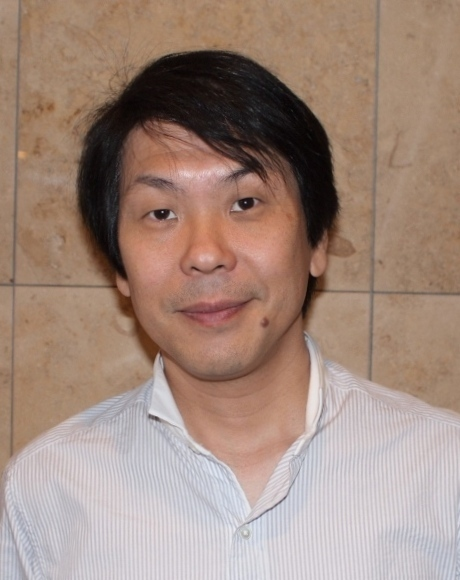
\includegraphics[height=1.5cm]{figs/Inoue-sensei.jpg} \\ \tval{Katsumi INOUE} \\ Professor \& team leader
  \end{tabular}}\right\}\text{\tval{Inoue Laboratory}}$
  &
  $\left.\text{\begin{tabular}{c}
    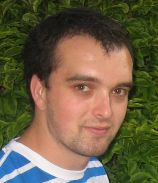
\includegraphics[height=1.5cm]{figs/Loic.jpg} \\ \tval{Loïc PAULEVÉ} \\ CNRS Researcher
  \end{tabular}}\right\}\text{\tval{Bioinfo}}$
  \\ & \\ & \\
  \multicolumn{2}{l}{$\left.\text{\begin{tabular}{ccc}
      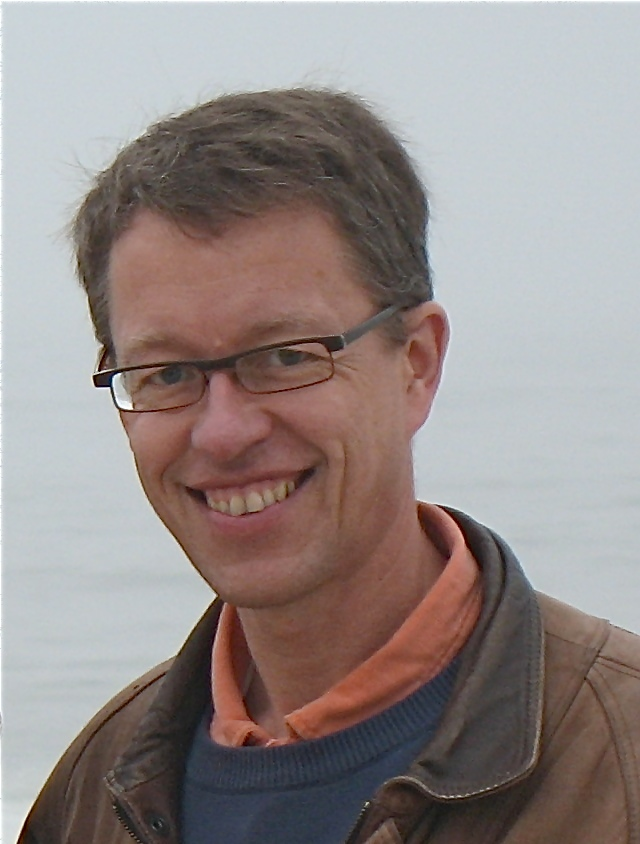
\includegraphics[height=1.5cm]{figs/Olivier.jpg}
    & 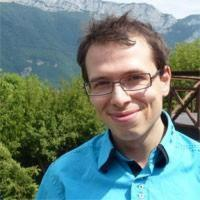
\includegraphics[height=1.5cm]{figs/Morgan.jpg}
    & 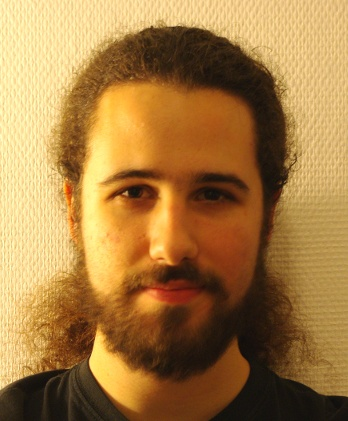
\includegraphics[height=1.5cm]{figs/Moi.jpg} \\
      \tval{Olivier ROUX} & \tval{Morgan MAGNIN} & \tval{Maxime FOLSCHETTE} \\
      Professor \& team leader & Associate professor & 2\textsuperscript{nd} year PhD student
  \end{tabular}}\right\}\text{\tval{MeForBio}}$}
\end{tabular}
\end{frame}

\appendix
\section[x]{Bibliography}
% Bibliographie

\begin{frame}[c]
  \frametitle{Bibliography}

\footnotesize
\setlength{\parindent}{-1em}
\setlength{\parskip}{0.5em}
~

\vfill

\tcite{PMR10-TCSB} Loïc Paulevé, Morgan Magnin, Olivier Roux. \ex{Refining dynamics of gene regulatory networks in a stochastic $\pi$-calculus framework}. In Corrado Priami, Ralph-Johan Back, Ion Petre, and Erik de Vink, editors: \textit{Transactions on Computational Systems Biology XIII}, volume 6575 of Lecture Notes in Computer Science, 171-191. Springer Berlin/Heidelberg, 2011.

\tcite{PMR12-MSCS} Loïc Paulevé, Morgan Magnin, Olivier Roux. \ex{Static analysis of biological regulatory networks dynamics using abstract interpretation}. \textit{Mathematical Structures in Computer Science}, 2012.

%\tcite{RCB08} Adrien Richard, Jean-Paul Comet, Gilles Bernot. \ex{R. Thomas' logical method}, 2008. Invited at \textit{Tutorials on modelling methods and tools: Modelling a genetic switch and Metabolic Networks}, Spring School on Modelling Complex Biological Systems in the Context of Genomics.

\tcite{RCB06} Adrien Richard, Jean-Paul Comet, Gilles Bernot. \textit{Modern Formal Methods and App.}, chapter \ex{Formal Methods for Modeling Biological Regulatory Networks}, pages 83--122. 2006.


\tcite{CMSB12} Maxime Folschette, Loïc Paulevé, Katsumi Inoue, Morgan Magnin, Olivier Roux. \ex{Concretizing the Process Hitting into Biological Regulatory Networks}. In David Gilbert and Monika Heiner, editors, \textit{Computational Methods in Systems Biology X}, Lecture Notes in Computer Science, pages 166–186. Springer Berlin
Heidelberg, 2012.

%\tcite{Paulevé11} Loïc Paulevé. PhD thesis: \ex{\textit{Modélisation, Simulation et Vérification des Grands Réseaux de Régulation Biologique}}, October 2011, Nantes, France

%\tcite{PMR10-TSE} Loïc Paulevé, Morgan Magnin, and Olivier Roux. \textit{Tuning Temporal Features within the Stochastic $\pi$-Calculus}. IEEE Transactions on Software Engineering, 37(6):858-871, 2011.

%\tcite{PR10-CRAS} Loïc Paulevé and Adrien Richard. \textit{Topological Fixed Points in Boolean Networks}. Comptes Rendus de l'Académie des Sciences - Series I - Mathematics, 348(15-16):825 - 828, 2010.

\vfill
\Large
\begin{flushright}
  \tval{Thank you}\hspace{1cm}~
\end{flushright}
\vfill

~

\end{frame}

\section[Annex: Graphs of local causality]{Graphs of local causality}
%% Exemples de structures abstraites (graphes de causalité locale)



% Analyse statique

\subsubsection{Successive reachability}

\begin{frame}
  \frametitle{Static analysis: successive reachability}
  \framesubtitle{\tcite{\cpmrmscs}}

Successive reachability of processes:

\begin{columns}
\begin{column}{0.55\textwidth}

\begin{center}
\scalebox{0.75}{
\begin{tikzpicture}
%\path[use as bounding box] (-1,-3) rectangle (7,2);
\exatt

\TState{2-4}{a_0,b_0,b_2,c_0,d_0}

\TState{5}{a_0,b_0,c_0,d_0}
\TState{6}{a_0,b_0,c_1,d_0}
\TState{7}{a_0,b_0,c_1,d_1}
\TState{8}{a_0,b_1,c_1,d_1}
\TState{9}{a_0,b_1,c_1,d_2}

\node<3>[process,very thick] (d_1) at (d_1.center) {1?};
\node<3>[process,very thick] (b_1) at (b_1.center) {2?};
\node<3>[process,very thick] (d_2) at (d_2.center) {3?};

\node<4-8>[process,very thick] (d_2) at (d_2.center) {1?};
\node<9>[process,very thick] (d_2) at (d_2.center) {};

\only<5>{\THit{a_0}{hlhit}{c_0}{.north}{c_1}}
\path<5>[bounce,bend left,hlhit] \TBounce{c_0}{}{c_1}{.west};
\only<6>{\THit{b_0}{hlhit}{d_0}{.west}{d_1}}
\path<6>[bounce,bend left,hlhit] \TBounce{d_0}{}{d_1}{.south};
\only<7>{\THit{c_1}{bend left=20pt,hlhit}{b_0}{.west}{b_1}}
\path<7>[bounce,bend left,hlhit] \TBounce{b_0}{}{b_1}{.south};
\only<8>{\THit{b_1}{hlhit}{d_1}{.west}{d_2}}
\path<8>[bounce,bend left,hlhit] \TBounce{d_1}{}{d_2}{.south};
\end{tikzpicture}
}
\end{center}

\end{column}
\begin{column}{0.45\textwidth}

\pause
~\\~\\~\\~\\
\begin{itemize}
  \item Initial context
    \\ \rex{\PHetat{a_1, \{b_0, b_1\}, c_0, z_0}} \pause
  \item Objectives
    \\ \rex{$[\ \Rsh d_1 \PHconcat\ \Rsh b_1 \PHconcat\ \Rsh d_2\ ]$} \pause
    \\\smallskip \rex{$[\ \Rsh d_2\ ]$} \pause
\end{itemize}

\end{column}
\end{columns}

\medskip
\begin{center}
\f Concretization of the objective = scenario

\ex{
\only<5>{\underline{$\PHfrappe{a_0}{c_0}{c_1}$}}\only<-4,6->{$\PHfrappe{a_0}{c_0}{c_1}$}~\PHconcat~
\only<6>{\underline{$\PHfrappe{b_0}{d_0}{d_1}$}}\only<-5,7->{$\PHfrappe{b_0}{d_0}{d_1}$}~\PHconcat~
\only<7>{\underline{$\PHfrappe{c_1}{b_0}{b_1}$}}\only<-6,8->{$\PHfrappe{c_1}{b_0}{b_1}$}~\PHconcat~
\only<8>{\underline{$\PHfrappe{b_1}{d_1}{d_2}$}}\only<-7,9->{$\PHfrappe{b_1}{d_1}{d_2}$}}
\end{center}

\end{frame}



\begin{frame}
  \frametitle{Over- and Under-approximations}
  \framesubtitle{\tcite{\cpmrmscs}}

Static analysis by abstractions:
\begin{fleches}
  \item Directly checking an objective sequence $R$ is hard
  \item Rather check the approximations $P$ and $Q$, where \tval{$P \Rightarrow R \Rightarrow Q$}:
\end{fleches}

\begin{center}
\scalebox{0.6}{
\figsa
}
\end{center}

\only<-7>{~}
\only<8->{
Polynomial w.r.t.~the number of sorts and \\exponential w.r.t.~the number of processes in each sort
\begin{fleches}
  \item Efficient for big models with few levels of expression
\end{fleches}
}
\end{frame}



\begin{frame}[c]
  \frametitle{Implementation \& Execution times}

\Pint\tval{: Existing free OCaml library}

\medskip
\f Compiler + tools for Process Hitting models

\f Documentation \& examples: \lien{http://processhitting.wordpress.com/}

\pause
\bigskip
\medskip
\tval{Computation time for various reachability analyses:}

\medskip
\small
\begin{tabular}{r||c|c|c|c||c|c|c|}
\hline
\tval{Model} & Sorts & Procs & Actions & States & Biocham$^1$ & libddd$^2$ & \Pint \\\hline
\tval{\ex{egfr20}} & 35 & 196 & 670 & $2^{64}$ & [3s--$\infty$] & [1s--150s] & \tval{0.007s} \\\hline
\tval{\ex{tcrsig40}} & 54 & 156 & 301 & $2^{73}$ & [1s--$\infty$] & [0.6s--$\infty$] & \tval{0.004s} \\\hline
\tval{\ex{tcrsig94}} & 133 & 448 & 1124 & $2^{194}$ & $\infty$ & $\infty$ & \tval{0.030s} \\\hline
\tval{\ex{egfr104}} & 193 & 748 &  2356 & $2^{320}$ &  $\infty$ & $\infty$ & \tval{0.050s}\\\hline
\end{tabular}

\medskip
\quad$^1$ Inria Paris-Rocquencourt/Contraintes\\
\quad$^2$ LIP6/Move

\cmodels
\end{frame}




\begin{frame}
  \frametitle{Under-approximation}

\def \tu {2}
\def \tub {3}
\def \tuf {4}

\begin{columns}
\begin{column}{0.48\textwidth}

\begin{center}
\scalebox{0.55}{
\begin{tikzpicture}
  \exatt
  \TState{-\tu}{a_1,b_1,c_1,d_0}
  \TState{\tub-}{a_0,b_1,c_0,d_0}
  \node[objective] (d_2) at (d_2.center) {?};
\end{tikzpicture}
}
\end{center}

\end{column}
\begin{column}{0.52\textwidth}

\vspace{1.5em}
\tval{Sufficient condition}:

\smallskip
\begin{itemize}
  \item no cycle
  \item \only<-\tu>{each objective has a solution} \only<\tub->{\sout{each objective has a solution}}
\end{itemize}
\begin{center}
  \only<\tu>{\Large\textcolor{darkgreen}{$R$ is \textbf{true}}} \only<\tuf>{\Large\textcolor{darkyellow}{\textbf{Inconclusive}}}
\end{center}

\end{column}
\end{columns}

\begin{center}%
%\vspace*{1cm}%
\scalebox{\scaleex}{%
\only<-\tu>{%
\scalebox{\scaleex}{%
\begin{tikzpicture}[aS]
  \path[use as bounding box] (.7,1) rectangle (5.8,2.5);

  \glclegend{}{$d_2$}{$\PHobj{d_0}{d_2}$}
\end{tikzpicture}
}
  \sauyes
}
\only<\tub->{
  \sauinconc
}}
\end{center}
\end{frame}



\begin{frame}
  \frametitle{Over-approximation}

\def \to {4}
\def \tob {5}
\def \tof {6}
\def \tokp {7}

\begin{columns}
\begin{column}{0.48\textwidth}

\begin{center}
\scalebox{0.55}{
\begin{tikzpicture}
  \exatt
  \TState{-\to}{a_1,b_0,c_0,d_1}
  \TState{\tob-}{a_1,b_1,c_1,d_0}
  \node[objective] (d_2) at (d_2.center) {?};
\end{tikzpicture}
}
\end{center}
\bigskip

\end{column}
\begin{column}{0.52\textwidth}

\tval{Necessary condition}:

\smallskip
\only<2->{
\only<3-\to>{\sout{There exists a traversal}}\only<2,\tob->{There exists a traversal}
with no cycle

\smallskip
\begin{itemize}
  \item \only<3-\to>{\sout{objective $\rightarrow$ follow one solution}}\only<1-2,\tob->{objective $\rightarrow$ follow one solution}
  \item solution $\rightarrow$ follow all processes
  \item process $\rightarrow$ follow all objectives
\end{itemize}
\begin{center}
  \only<\to>{\Large\textcolor{red}{$R$ is \textbf{false}}}\only<\tof->{\Large\textcolor{darkyellow}{\textbf{Inconclusive}}}
\end{center}
}

\end{column}
\end{columns}

\begin{center}
\scalebox{\scaleex}{
\only<1-\to>{
  \saono
}
\only<\tob->{
  \saoinconc
}}
\end{center}
\end{frame}

%% Propriétés supplémentaires du Process Hitting

\section[Annex: Fixed Points]{Fixed Points}

\begin{frame}[c]
  \frametitle{Static Analysis: Fixed Points}
  \framesubtitle{\tcite{\cpmrtcsb}}

\tval{Fixed point} = state where no action can be fired
\begin{fleches}
  \item avoid couples of processes bounded by an action
\only<1>{\\\smallskip~}
\only<2->{\item Hitless Graph \only<3->{\f \tval{n-cliques} = fixed points}}
\end{fleches}

\bigskip
\begin{columns}
\begin{column}{0.5\textwidth}

\begin{center}
\scalebox{0.7}{
\begin{tikzpicture}
\exdefb
\exdefbfrappes
\end{tikzpicture}
}
\end{center}

\end{column}
\begin{column}{0.5\textwidth}

\only<2->{
\begin{center}
\scalebox{0.7}{
\tikzstyle{current process}=[process,fill=red]
\begin{tikzpicture}[hitless graph]
\exdefb
\exdefbsf
\end{tikzpicture}
\tikzstyle{current process}=[process,fill=blue]
}
\end{center}
}

\end{column}
\end{columns}

\bigskip
\pause[6]
Exponential complexity w.r.t.~the number of sorts

\end{frame}



\section[Annex: Stochastic Features]{Stochastic Features}

\begin{frame}
  \frametitle{Stochastic Features}
  \framesubtitle{\tcite{\cpmrtcsb}}

\begin{itemize}
  \item Introduces time features
  \item Parameters: either $(r,sa)$, or the \tval{firing interval} $[d;D]$.
\end{itemize}

\begin{columns}
\begin{column}{0.5\textwidth}

\only<2->{
\scalebox{0.9}{
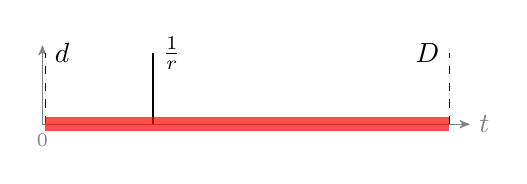
\begin{tikzpicture}[plot,xscale=0.35,yscale=1]
\draw[axe] (0,0) -- (15.5,0) node[right] {$t$};
\draw[axe] (0,0) -- (0,1);
\draw[ticks] (0,0) node[below] {$0$};
\draw[mean] (4,0) -- (4,0.9) node[right]{$\frac{1}{r}$};
\draw[dashed] (0.10127,0) -- (0.10127,0.9) node[right] {$d$} (14.75552,0) --
(14.75552,0.9) node[left] {$D$};
\pgfplothandlerlineto
\pgfplotxyfile{plots/BioAtlanSTIC-0409/erlang-0.25-1.table}
\pgfusepath{stroke}
\draw[interval] (0.10127,0) -- (14.75552,0);
\end{tikzpicture}
}

\scalebox{0.9}{
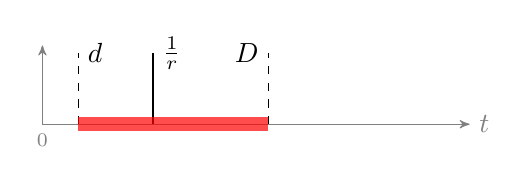
\begin{tikzpicture}[plot,xscale=0.35,yscale=1]
\draw[axe] (0,0) -- (15.5,0) node[right] {$t$};
\draw[axe] (0,0) -- (0,1);
\draw[ticks] (0,0) node[below] {$0$};
\draw[mean] (4,0) -- (4,0.9) node[right]{$\frac{1}{r}$};
\draw[dashed] (1.29879,0) -- (1.29879,0.9) node[right] {$d$} (8.19327,0) --
(8.19327,0.9) node[left] {$D$};
\pgfplothandlerlineto
\pgfplotxyfile{plots/BioAtlanSTIC-0409/erlang-0.25-5.table}
\pgfusepath{stroke}
\draw[interval] (1.29879,0) -- (8.19327,0);
\end{tikzpicture}
}

\scalebox{0.9}{
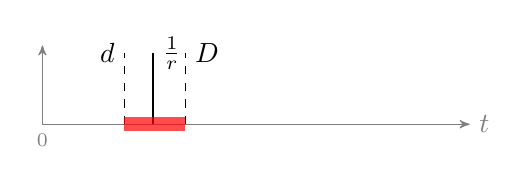
\begin{tikzpicture}[plot,xscale=0.35,yscale=1]
\draw[axe] (0,0) -- (15.5,0) node[right] {$t$};
\draw[axe] (0,0) -- (0,1);
\draw[ticks] (0,0) node[below] {$0$};
\draw[mean] (4,0) -- (4,0.9) node[right]{$\frac{1}{r}$};
\draw[dashed] (2.96888,0) -- (2.96888,0.9) node[left] {$d$} (5.18245,0) --
(5.18245,0.9) node[right] {$D$};
\pgfplothandlerlineto
\pgfplotxyfile{plots/BioAtlanSTIC-0409/erlang-0.25-50.table}
\pgfusepath{stroke}
\draw[interval] (2.96888,0) -- (5.18245,0);
\end{tikzpicture}
}

~~\textcolor{red!70}{\rule{17mm}{4.5pt}} ~ action duration
}

\end{column}
\begin{column}{0.5\textwidth}
\begin{center}

\only<3->{
\scalebox{0.9}{
\begin{tikzpicture}
\path[use as bounding box] (-1,-1) rectangle (2,1);
\TSort{(0,0)}{a}{2}{l}
\TSort{(2,0)}{b}{2}{r}
\THit{a_0}{}{b_0}{.west}{b_1}
\THit{a_0}{out=-120,in=180,selfhit}{a_0}{.west}{a_1}
\path[bounce]
\TBounce{a_0}{bend left}{a_1}{.south}
\TBounce{b_0}{bend left}{b_1}{.south}
;
\TState{3-}{a_0,b_0}
\end{tikzpicture}
}

\scalebox{0.9}{
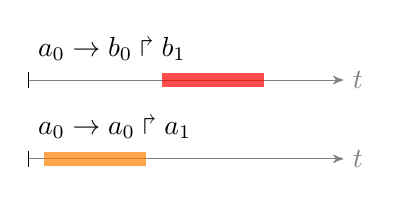
\begin{tikzpicture}[plot]
\node[anchor=west] at (0,0.4) {$\PHfrappe{a_0}{b_0}{b_1}$};
\draw[axe] (0,0) -- (4,0) node[right] {$t$};
\draw (0,0.1) -- (0,-0.1);
\draw[interval] (1.7,0) -- (3,0);

\node[anchor=west] at (0,-0.6) {$\PHfrappe{a_0}{a_0}{a_1}$};
\draw[axe] (0,-1) -- (4,-1) node[right] {$t$};
\draw (0,-0.9) -- (0,-1.1);
\draw[interval,orange] (0.2,-1) -- (1.5,-1);
\end{tikzpicture}
}

\noindent
\f $b_1$ reached with a \tval{very low probability}.
}

\end{center}
\end{column}
\end{columns}

\pause[4]
\bigskip
\begin{fleches}
  \item Tests by simulation
  \item Model-checking
\end{fleches}

\end{frame}


\end{document}
